\documentclass{lutmscthesis}[2010/09/22]
%\documentclass[draft]{lutmscthesis}   % leave figures blank, faster

\usepackage[utf8]{inputenc}
\usepackage[T1]{fontenc}
\usepackage[english]{babel}

\usepackage{times}
\usepackage{tabularx}
\usepackage{multirow}

\usepackage{setspace}
\usepackage{verbatim}
\usepackage[intlimits]{amsmath}
\usepackage{enumitem}

\usepackage{pgfplots} 
\pgfplotsset{compat=newest} 
\newlength\figurewidth
\newlength\figureheight

% Ensure figure captions are below and table captions are above the content.
\usepackage{float}
\floatstyle{plain}\restylefloat{figure}
\floatstyle{plaintop}\restylefloat{table}

\usepackage[pdfborder={0 0 0}]{hyperref}
%\usepackage[]{algorithm}
\usepackage[ruled]{algorithm2e}

\usepackage{cite}


%           Hyperref rationale - or just pain in the butt
%
% Load 'float' package first, because that will fix problems with 'algorithm'
% package interacting with hyperref.
%
% Hyperref must be the last package loaded, except...
% Load 'algorithm' AFTER hyperref, otherwise \theHalgorithm is
% undefined control sequence error appears.
%
% The TeXLive 2008 version of 'algorithmic' is buggy with hyperref.
% Use this bundled, special, hand-fixed version of algorithmic.sty
% instead. It is identified by version 2006/12/15.


\graphicspath{{resources/}}

\newcommand{\vect}[1]{\boldsymbol{#1}}
\newcommand{\matr}[1]{\boldsymbol{#1}}
\newcommand{\diag}[1]{\mathrm{diag}(#1)}
\newcommand{\iprod}[1]{\left\langle #1 \right\rangle}
\newcommand{\me}{\mathrm{e}}
\newcommand{\mi}{\mathrm{i}}
\newcommand{\md}{\mathrm{d}}
\newcommand{\sse}{{}} %\mathrm{SSE}}
\newcommand{\trace}{\mathrm{Tr}\:}
\newcommand{\frp}[2]{{}^\mathrm{#1}\vect{#2}}
\newcommand{\frs}[3]{{}^\mathrm{#1}#2_\mathrm{#3}}
\newcommand{\frv}[3]{{}^\mathrm{#1}\vect{#2}_\mathrm{#3}}
\newcommand{\frm}[3]{{}^\mathrm{#1}\matr{#2}_\mathrm{#3}}
\newcommand{\colvec}[2]{\genfrac{[}{]}{0pt}{1}{#1}{#2}}
\newcommand{\relphantom}[1]{\mathrel{\phantom{#1}}}
\newcommand\aug{\fboxsep=-\fboxrule\!\!\!\fbox{\strut}\!\!\!}

\newcommand{\etal}{\textit{et al}. }

\newtheorem{theorem}{Theorem}



% Thesis information

\title{Contour segment grouping for overlapping convex object segmentation}

\author{Nikita Ashikhmin}

\Faculty{School of Engineering Science \\ Master's Programme in Computational Engineering and Technical Physics}
\Major{Intelligent Computing Major}

\Keywords{segment grouping, convex object segmentation, concavity analysis, seed point, fast radial symmetry, image processing, image analysis}

\Supervisors{
M.Sc. (Eng.) Sahar Zafari \\
Adjunct Professor, Dr. Tuomas Eerola \\
Dr. Jouni Sampo \\
Prof. Heikki Kälviäinen
}
\Examiners{Professor Heikki K\"alvi\"ainen \\Associate Professor, Cand. Sci Gleb Radchenko}

\Year{2017}

% Thesis statistics: figure, table and appendix counts, for abstracts
\addtostats{, 19 figures, 2 tables, 2 appendixes}

\begin{document}
\selectlanguage{english}

\maketitle
\newpage

\begin{abstract}
Segmentation of overlapping convex object has many real-world applications, including material analysis and morphological analysis of biological cells. The methods for convex object segmentation usually consist of the following stages: 1) edge detection, 2) edge segmentation, 3) segment grouping, and 4) estimating the full contours of the objects. 
This thesis presents an overview of methods and approaches that are used for convex object segmentation. This thesis is focused on the segment grouping part. The novel proposed method is based on estimating a shell, which covers all segments of the group and has minimal area. The proposed segment grouping method was compared with current state-of-art segment grouping method on two types of data: synthetic data and real data. The synthetic data consists of images with different triangle, quadrilateral, ellipse particles. The real data consist of nanoparticles images captured using transmission electron microscopy and marked manually. The results of experiments shown that the proposed segment grouping method shows improved results on images with shapes of different types. 
\end{abstract}


%\begin{preface}
%Lappeenranta, \today
%\end{preface}


% These name-definitions must be after Babel language change
% commands, as they redefine these.
\renewcommand\refname{REFERENCES}
\renewcommand\contentsname{CONTENTS}

\pagestyle{masters}
\newpage


% ---------------------------------------
%           TABLE OF CONTENTS
% ---------------------------------------

\tableofcontents


% ---------------------------------------
%    LIST OF SYMBOLS AND ABBREVIATIONS
% ---------------------------------------

\section*{LIST OF ABBREVIATIONS}

\begin{tabular}{l l}
ADD &  Average Distance Deviation Criteria\\
ARF & Adaptive Ring Filter\\
BB & Branch and Boundaries\\
BE-FRS & Bounded-Erosion Fast Radial Symmetry\\
CF & Coin Filter\\
CSS & Curvature Scale Space \\
DT & Distance Transform \\
FRS & Fast Radial Symmetry \\
IF & IRIS Filter\\
LCF & Local Convergence Filter\\
MMM & Maximum-Match-Measure\\
SBF & Sliding Band Filter\\
UE & Ultimate Erosion\\
UECS & Ultimate Erosion for Convex Sets\\
\end{tabular}



% space between paragraphs
\setlength{\parskip}{3ex}


% ---------------------------------------
%             INTRODUCTION
% ---------------------------------------

\section{INTRODUCTION}
\label{sec:introduction}

\subsection{Background}
\label{sec:background}

Segmentation or contour estimation of overlapping objects is an image analysis task. This task is connected to the problem of analyzing 2D projections of 3D objects. It is widely used in the industry and biology. Usually, it is difficult to estimate inner contours of the overlapped object so the segmentation methods must relay just on visible parts of particles (see Figure~\ref{fig:real_data}). To solve such problems one must estimate the full contour based on visible edge fragments and prior knowledge about the object shape~\cite{zafari-thesis}.

\begin{figure}[ht]
  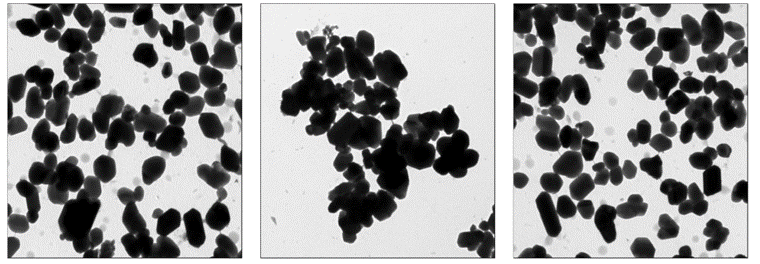
\includegraphics[width=\linewidth]{real_data.png}
  \caption{Examples of images from transmission electron microscopy.}
  \label{fig:real_data}
\end{figure}

This work focuses on segmentation of convex objects. The work continues earlier research where a framework to segment (estimate contours) of partially overlapping nanoparticles was developed~\cite{zafari2017comparison}. The framework consists of three steps: 
1) detecting of concave edge points, 
2) grouping of the resulting edge segments to form contour evidence, and 3) estimating the full contours of the objects (see Fig.~\ref{fig:concave_framework})~\cite{Zafari15,zafari-bb}.

\begin{figure}[ht]
  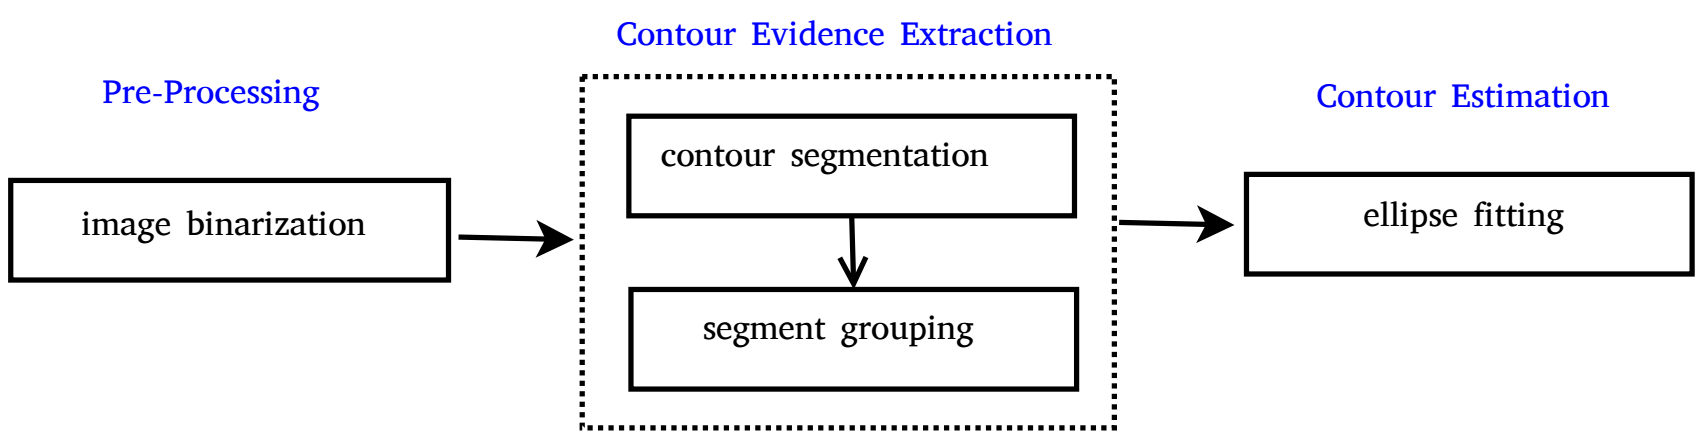
\includegraphics[width=\linewidth]{concave-framework.png}
  \caption{Concave points based framework.~\cite{zafari-bb}}
  \label{fig:concave_framework}
\end{figure}

In order to be able to estimate full contours of objects with partially observed edges, all edge points or edge segments belonging to the same object need to be grouped. To do this, shape analysis of the resulting object is needed. This can be done by employing a grouping method that defines how likely two edge segments belong to the same object, that is how well the resulting object fits the prior information about the object shapes or contour model. 


\subsection{Objectives and delimitations}
\label{sec:objectives}

The aim of this master’s thesis is to develop an efficient grouping strategy that grouping the contour segments which belong to the same object.

The objectives are as follows:
\begin{enumerate}
\item Make an overview of existing methods and frameworks for overlapping object segmentation.
\item Propose the new segment grouping method, that improves the performance of segment grouping on images with shapes of different types.
\item Compare the proposed method with existing state-of-art segment grouping method on real and generated data.
\end{enumerate}



\subsection{Structure of the thesis}

The rest of thesis has the following structure. Chapter 2 gives a brief overview of an existing contour segmentation methods. This chapter contains a description of seed point extraction methods, concave point-based methods, and edge segment grouping methods. Chapter 3 presents a segmentation framework with a new proposal of a segment grouping method. Chapter 4 contains the information about experiments and validation of the proposed segment grouping method. Chapter 5 discusses the findings and describes goals of the further research. Chapter 6 concludes the thesis and give a brief overview of the problem, the solution, and the results.

% ---------------------------------------
%             RELATED WORK
% ---------------------------------------

\section{SEGMENTATION OF OVERLAPPING CONVEX OBJECTS}
\label{sec:related}

There are two typical approaches to solve the segmentation of overlapping convex object segmentation problem. The first approach is based on the extraction of seed points~\cite{zafari-thesis}, special points, that are geometrical centers of overlapping objects. The second approach is based on concave point detection~\cite{Zafari15}. This method extracts visible boundaries of overlapping objects and detects the special concave points that are corners between overlapping objects.  

\subsection{Seed point-based methods}

The seed point extraction is one of the most important steps. It has a big impact on the accuracy of the final segmentation result. Seed point extraction produces a priori information that is used in counter evidence extraction and contour estimation. The goal of this step is to recognize the number of the individual overlapping objects in the image and correspond them with seed points. 

A  seed point-based framework for segmentation of overlapping object consists of the next specific steps~\cite{zafari-thesis}:


\begin{enumerate}
\item Seed region/point extraction. In this step, there is extracting points or regions of each overlapping object. The seed points usually refer to a geometrical center point of anticipated overlapping objects. The goal of this step is to recognize the number of the individual overlapping objects. The count and position of the detected points in this step are not final and can be improved during the next steps.
\item Contour evidence extraction is the determination of the counter evidence, the visible parts of the object boundaries, that are used to determinate the hide parts of overlapped objects. The aim of this step to group edge points that belong to each object using information about seed points or seed region from the previous step.
\item Contour estimation. The full contour of all overlapping objects is estimated based on results of the previous steps.
\end{enumerate}


The schema of the framework is shown in Figure~\ref{fig:general_framework}.

\begin{figure}[ht]
  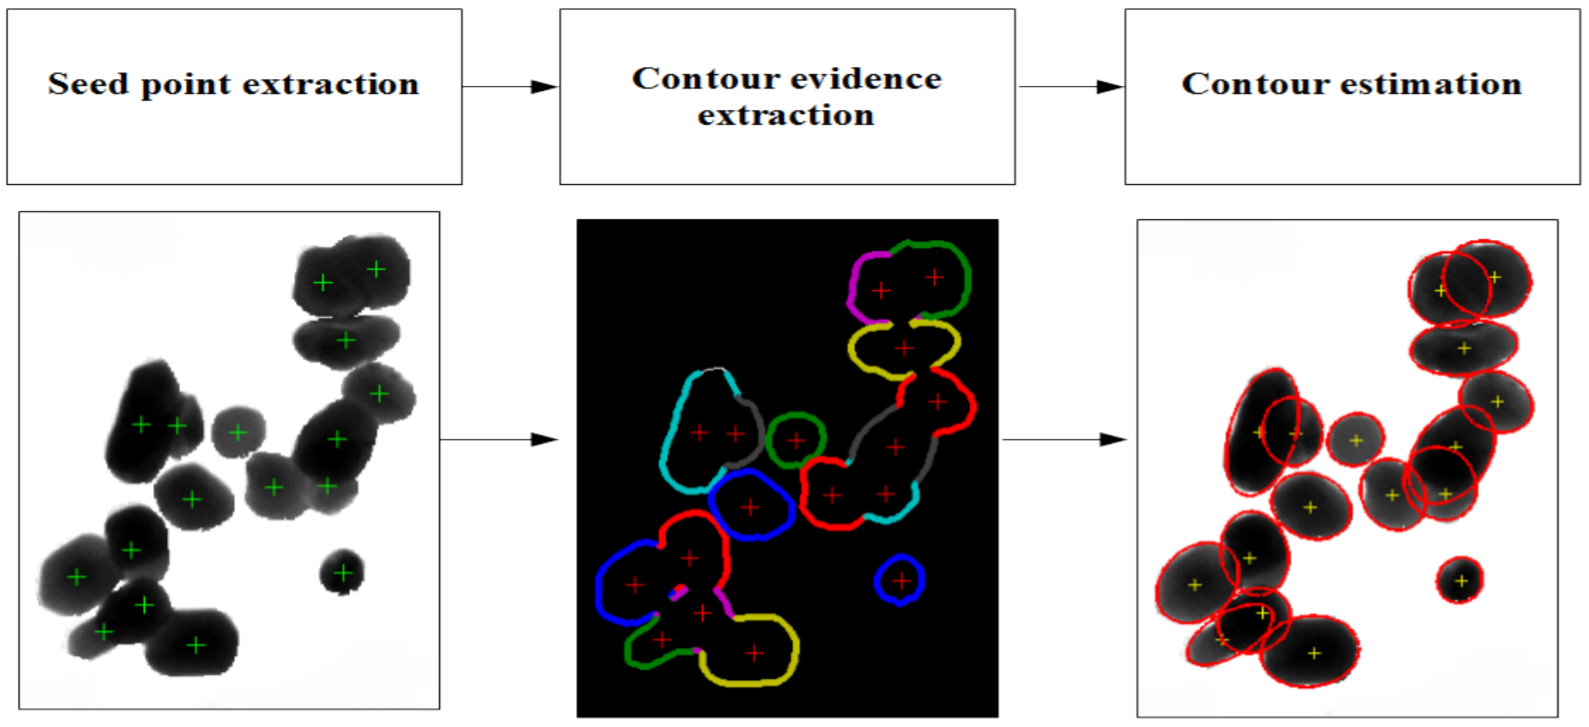
\includegraphics[width=\linewidth]{General_framework.png}
  \caption{Framework based on seed points.~\cite{zafari-thesis}}
  \label{fig:general_framework}
\end{figure}

There is a lot of different approaches for seed point extractions, such as Local Convergence Filters~\cite{LCF}, Ultimate Erosion for Convex Sets~\cite{UECS}, Distant Transform~\cite{DT}, Fast radial symmetry~\cite{BE-FRS}.


\subsubsection{Local Convergence Filters}
The description of the local coverage filters is based on~\cite{LCF}.
Local Convergence Filters (LCF)~\cite{LCF} are seed points extraction methods, based
in gradient convergence and tolerant to noise, illumination variations, and low contrast.
This group of filters is one of the most used algorithms to detect seed points.
The idea of these algorithms to detect regions in the image with converges of a gradient, what is proper for searching convex shapes. 
Local Convergence Filters determinate a scale for shape detection and perform
detection based on the response within an area relating to
such scale, so-called support region. Moreover, LCF have the good robustness to noise due to the essentially added shape prior. The differ between variations of LCF is a shape of a support region. The examples of such filters are following: Coin Filter~\cite{LCF_CF}, IRIS filter~\cite{LCF_CF}, Adaptive Ring Filter~\cite{LCF-ARF}, Sliding Band Filter~\cite{LCF-SBF}. They are shown in Figure~\ref{fig:LCF-alg}.

\begin{figure}[ht]
  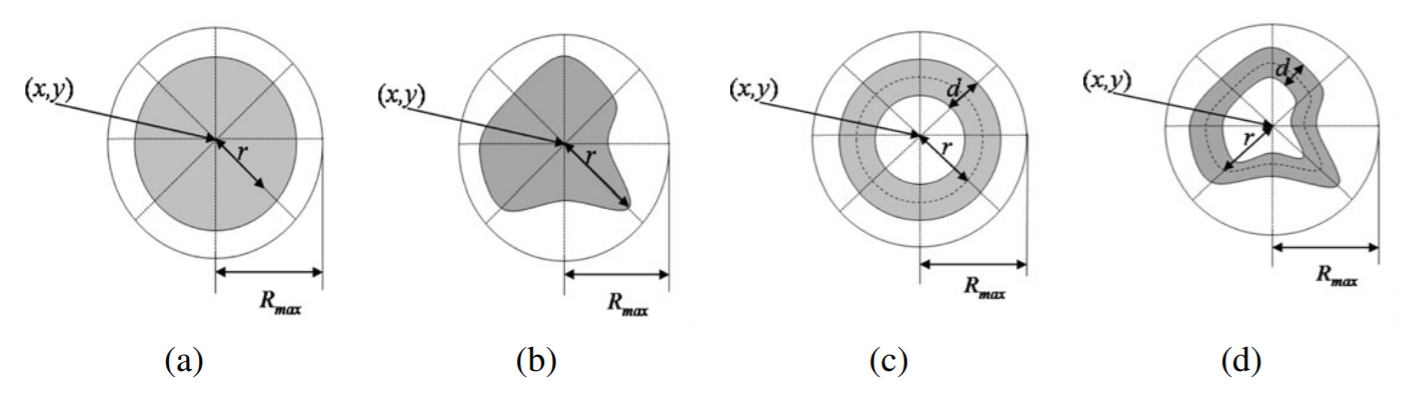
\includegraphics[width=\linewidth]{LCF.png}
  \caption{LCF filters: (a) Coin filter; (b) IRIS filter; (c) Adaptive ring filter; (d) Slide band filter.~\cite{LCF}}
  \label{fig:LCF-alg}
\end{figure}


\textit{\textbf{Coint Filter (CF)}}~\cite{LCF_CF} is the basic LCF method. The support region in this method has a circular shape. The value of the radius is varied in search for the one which
corresponds to maximum convergence, limited by a maximum
radius. 

\textit{\textbf{IRIS filter (IF)}}~\cite{LCF_CF} is a modification of the CF filter. The differs from the previous one in that the radius of a support region for every direction changing independently. As a result, this filter is not restricted to circular shapes and can handle more complex objects. 


\textit{\textbf{Adaptive Ring Filter (ARF)}}~\cite{LCF-ARF} define a ring-shaped convergence region. The motivation for that support
region is the idea that the convergence of a convex
objects is mostly originated at edges, which makes the method more noise-resistant.


\textbf{\textit{Sliding Band Filter (SBF)}}~\cite{LCF-SBF} unites both limited band search of ARF and the shape flexibility of IF. 
The result of work of SBF looks like the result of IRIS but provides better separating of overlapping objects.


Local Convergence Filters have one common shortcoming. These methods are based just on gradient orientation and ignore gradient magnitude that can lead to big segmentation errors when gradient magnitude
is low~\cite{LCF}. 



\subsubsection{Ultimate Erosion for Convex Sets}

Ultimate Erosion for Convex Sets (UECS)~\cite{UECS} is an iterative morphological algorithm that extracts
the seed regions from overlapping object. UECS is an extension of the Ultimate Erosion
(UE) method with a modified stopping criteria~\cite{UECS}. The algorithms consist of two stages. In the first stage, the image is decomposed into disjoint convex sets. This stage is based on the Ultimate Erosion algorithm with a modified stooping criteria that make possible to avoid over-segmentation. The result of this stage is set of disconnected objects.
The detailed visualization of the steps of the algorithm is shown in Figure \ref{fig:UECS-alg}.

\begin{figure} [ht]
  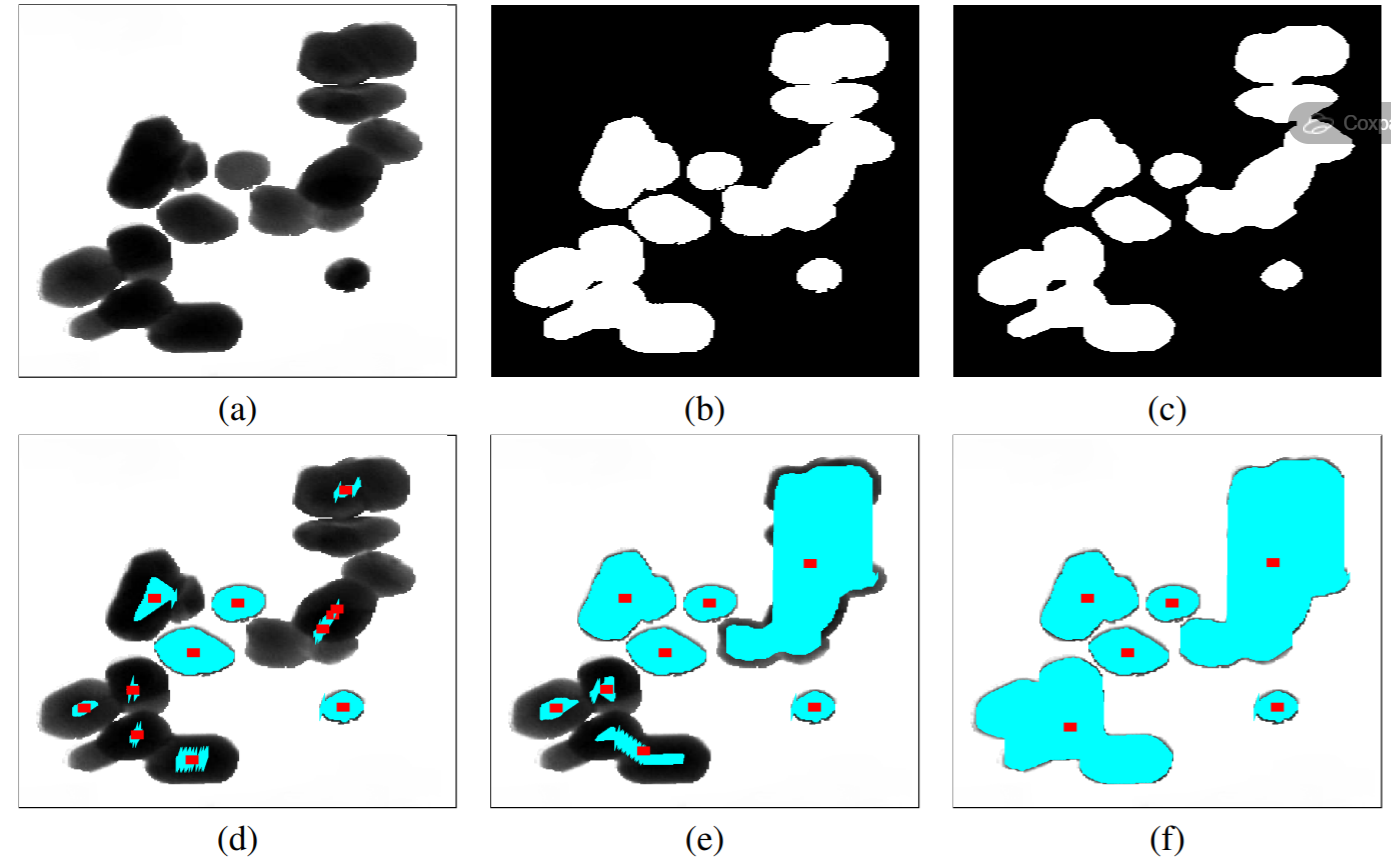
\includegraphics[width=\linewidth]{UECS.png}
  \caption{UECS seed point extraction: (a) Original image; 
    (b) Binary image; 
    (c) Binary image after morphological opening; 
    (d) Seed points identified with the threshold 0.1;
    (e) Seed points identified with the threshold 0.2;
    (f) Seed points identified with the threshold 0.3.~\cite{zafari-thesis}}
  \label{fig:UECS-alg}
\end{figure}

\subsubsection{Distance Transform}

Distance Transform (DT)~\cite{DT} is a simple operator applied to binary images. An output of the transform is a gray level image the same size with an original image, where each original white pixel contains distance to the closest boundary.t.
The method is visualized in Figure~\ref{fig:DT_img}. Algorithm~\ref{alg:DT} shows the main steps of the method.

\begin{algorithm} [H]
   \begin{enumerate}
        \item Binarization of the image;
        \item Morphological opening of the image;
        \item Interactively mapping of the value each pixel to the minimum value of the pixel area by DT;
        \item The seed point and region estimation by the predefined threshold;
    \end{enumerate}
    \caption{Distance Transform filter~\cite{DT-bactery}.}\label{alg:DT}
\end{algorithm}

\begin{figure} [ht]
  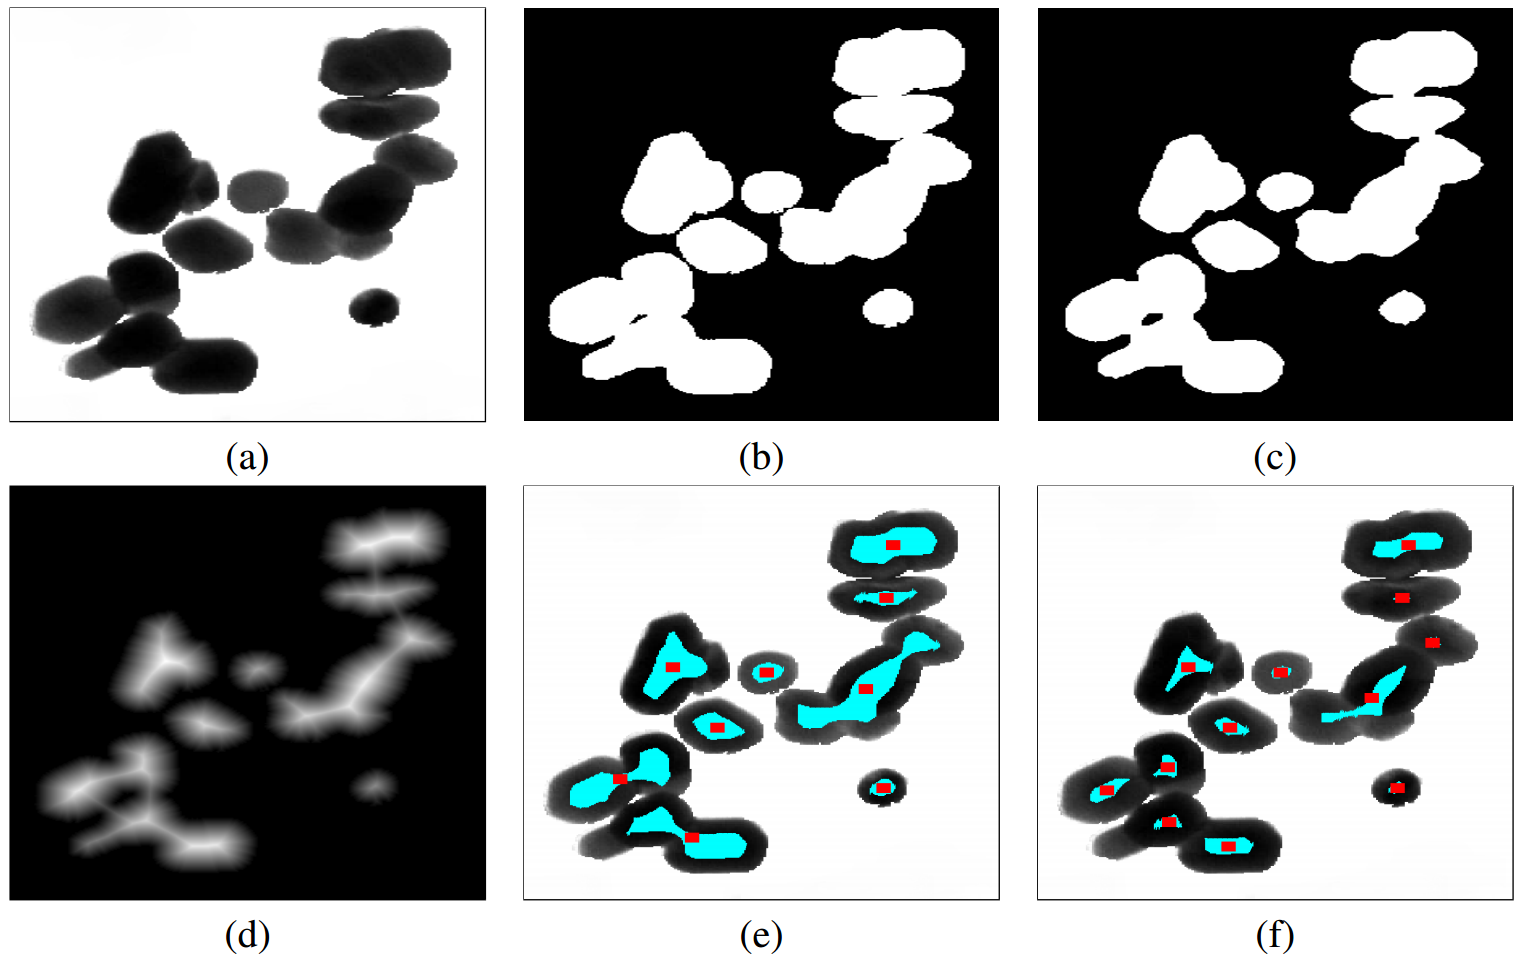
\includegraphics[width=\linewidth]{DT.png}
  \caption{
    Distance Transform seed point extraction: (a) Original image; (b) Binary image;
    (c) Binary image after morphological opening; 
    (d) Result of DT; 
    (e) Seed points identified with the threshold 0.6; 
    (f) Seed points identified with the threshold 0.7~\cite{zafari-thesis}.}
  \label{fig:DT_img}
\end{figure}


\subsubsection{Fast radial symmetry}

Fast radial symmetry (FRS)~\cite{FRS}  is a wide-used method that transforms the original
image to a new representation, highlighting the local radial symmetry of the image gradient.
The main idea pf FRS that  every edge pixel in the image giving a vote for the plausible radial symmetry at some specific distance from that point. This step relies on two parameters $R$ and $T$. $R = [R_{min} , R_{max}]$ represents the range of the vote of each point, and $T$ indicates the threshold for the distance between two adjacent seed points. The center
of gravity of each vote region is taken as its seed point which is used to mark
each object in the image. 

The current state-of-art technique in seed point extraction of elliptical objects is Bounded Erosion Fast
Radial Symmetry method (BE-FRS)~\cite{BE-FRS}, which is a modification of original FRS method. This technique uses two common properties of elliptical objects: convexity and symmetry.
It uses a hybrid model consisting of morphological erosion and FRS in a
silhouette image to obtain the seed points of each object, while each seed point
is used to mark an individual object. Applying bounded erosion~\cite{BE} before FRS improves the quality of seed point extraction by smoothing the shapes of overlapped objects.

\subsubsection{Edge to seed point watching}

The edge-to-marker association method~\cite{edge-to-seed-point} attach found seed points with visible edges of overlapped objects. This method is based on calculating \textit{a relevance metric} that combines the divergence metrics  and the distance from an edge pixel to a seed point. If $S ={s_1,s_2,...,s_n}$ is a set of seed points and $E ={e_1,e_2,...,e_n}$ is a set of edge points, a relevance metric for edge point $e_i$ and seed point $s_j$ can be calculated by the following formula:

\begin{equation}
    rel(e_i,s_j) = \frac{1-\lambda}{1+dist(e_i,s_j)}+\lambda\frac{div(e_i,s_j)+1}{2},
\end{equation} where $dist(.,.)$ is Euclidean distance and $div(.,.)$ is divergence functions respectively. Each function normalized to (0,1] and summed by $\lambda$ weight coefficient. In this way, the edge
point $e_i$ is assigned to seed point $s_j$ with the highest relevance
value (see Figure~\ref{fig:seed-point-assoc}).


\begin{figure} [ht]
  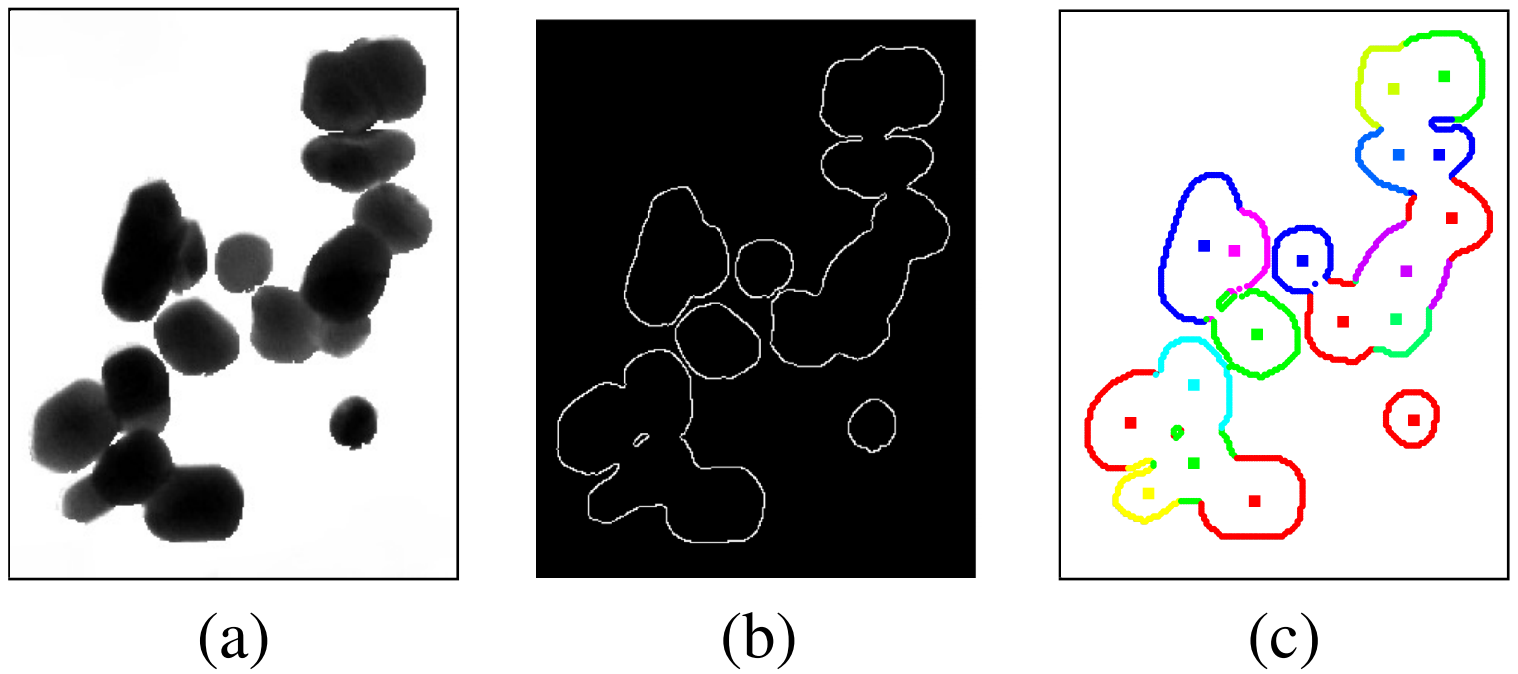
\includegraphics[width=\linewidth]{edge-to-seed-points.png}
  \caption{Edge to Seed points association: 
        (a) Original image; 
        (b) Visible contours of particles; 
        (c) Associations between seed points and contours.~\cite{BE-FRS}
    }
  \label{fig:seed-point-assoc}
\end{figure}

\subsection{Concave point-based methods}
Another approach for segmentation of overlapping objects is the concave point-based method~\cite{compare-cpd,Saddik,Zafari15}. The idea of this methods is dividing the contour of the group of overlapping objects to set of segments separated by special points, so-called concave points. The main steps of the methods are shown in Algorithm~\ref{alg:CPD}. The visualization of the method is shown in Figure~\ref{fig:Contour-segmentation}.

\begin{algorithm} [H]
    \begin{enumerate}
        \item Image binarization, for example, using Otsu method~\cite{otsu}.
        \item Dividing the image into the separate Regions of Interest (ROI)~, that contains particles or groups of overlapping particles.
        \item Extraction of the contour of the whole ROI~\cite{ROI}.
        \item Splitting the contour to the edges by extracting the concave points.
        \item Grouping of segments that are parts of one particle.
        \item Estimating the full contour of the object using, for example, ellipse fitting.
    \end{enumerate}
    \caption{Concave point-based method~\cite{Zafari15}.}\label{alg:CPD}
\end{algorithm}

\begin{figure} [ht]
  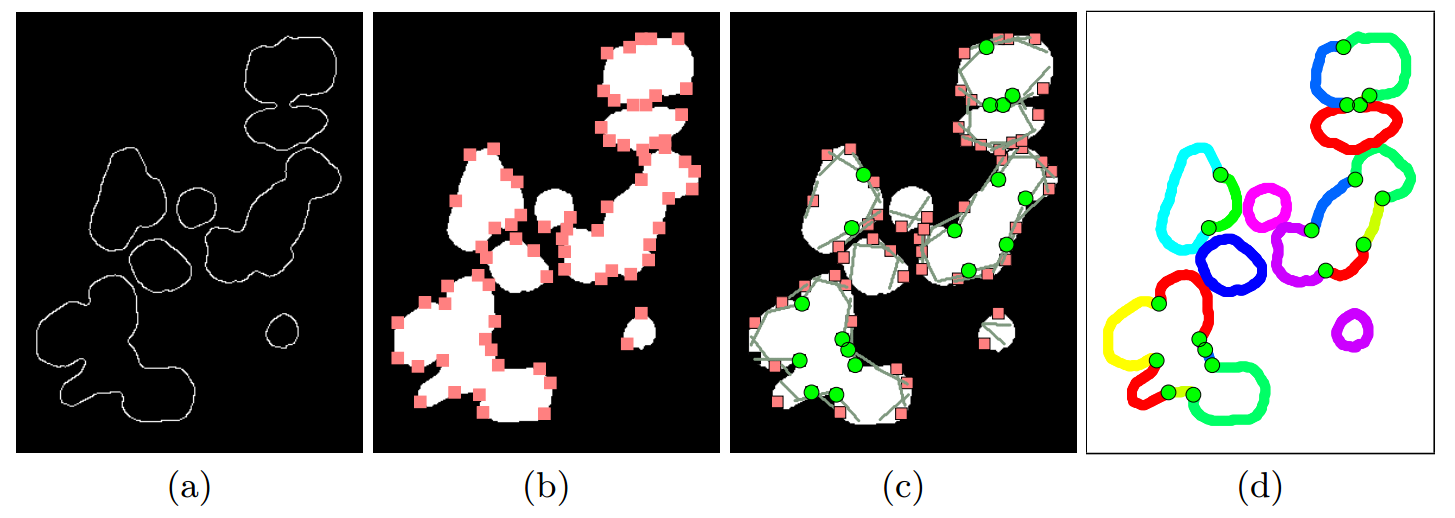
\includegraphics[width=\linewidth]{concave_points.png}
  \caption{: Contour segmentation: 
    (a) Counter map; 
    (b) Corner detection; 
    (c) Concavity points extraction;
    (d) Contour segmentation.~\cite{Zafari15}}
  \label{fig:Contour-segmentation}
\end{figure}




\subsubsection{Edge segmentation}
Edge segmentation is typically performed by detecting concave points.
The following methods exist for concave point detection~\cite{compare-cpd}:
\begin{enumerate}
    \item 
    \textit{Curvature based methods}. 
    These methods relate to an each edge pixel $(x_i,y_i)$ a special value, so-called \textit{curvature value}~\cite{Zafari15}.
    
    
    Furthermore, methods select special dominant points which are local extrema for curvature values. There are different strategies to pick over concave points from the set of dominant points. The method purposed by Wen \emph{et al.}~\cite{curv-wen}  select the points by a preset threshold, Zafari \emph{et al.}~\cite{Zafari15} approach is based choosing points that neighbors do not reside inside the object. Dai \emph{et al.}~\cite{curv-dai} present the method that calculates the triangle area of a point with neighbors and if the value of the area is positive the method marks the point as a concave point.
   
    \item 
    \textit{Skeleton methods}. This group of methods uses the skeleton and boundary information. The idea of method proposed by Samma~\emph{et al.}~\cite{bnd-skeleton} is the identification of concave points by computing the intersection between the skeleton and contour points. The method proposed by Wang \emph{et al.}~\cite{skeleton} detects concave points if the shortest distance to skeletons is more than a preset threshold.
    \item 
    \textit{Chord methods}. The main idea of these methods is the identification of concave points as points that have the maximum distance to the concave area chord. There are several methods to estimate concave point area which are described in 
    ~\cite{chord-farhan,chord-kumar}.
    
    \item 
    \textit{Polygon methods}. These groups of methods are a well-known way to represent the contour of the element as a sequence of dominant points. A dominant point is a contour point that does not lie on the line between its' neighbors. A concave point is a dominant point if the line between neighbors dominant points does not pass throw inside the object and the angle between these points is in the range of predefined thresholds~\cite{Bai20092434}. Zhang~\emph{et al.}~\cite{bubble} define a dominant point as a concave if scalar product between lines, that connect the dominant point with neighbor left and right points, is positive. Sahar~\emph{et al.}~\cite{compare-cpd} unite two methods~\cite{bubble} and~\cite{Bai20092434} to avoid any predefined parameters of the concave point detector.
\end{enumerate}
\subsubsection{Segment grouping}
The next step is grouping such segments which belong to one object, as shown in Figure~\ref{fig:Segment-grouping}. 
The naive edge segment grouping algorithm~\cite{bubble} iterates over each pair of contour segment, checking if they can be united in one ellipse. However, the number of ways to partition a set of $n$ segments into $p$ groups is very big according to the Stirling number formula:
\begin{equation}
    P(n,p) = \frac{1}{p!}\sum_{n_1+n_2+...+n_p=n}\frac{n!}{n_1!...n_p!},
\end{equation}
which means that brute-force algorithm is time-consuming.

Zhang~\emph{et al.}~\cite{bubble} proposed an average distance deviation criterion (ADD) as a metric for segment grouping. ADD is based on a heuristic that all particles have elliptical shapes. The method unites two groups of segments if the cost for each group is higher than the cost of merged groups.
\begin{figure} [ht]
  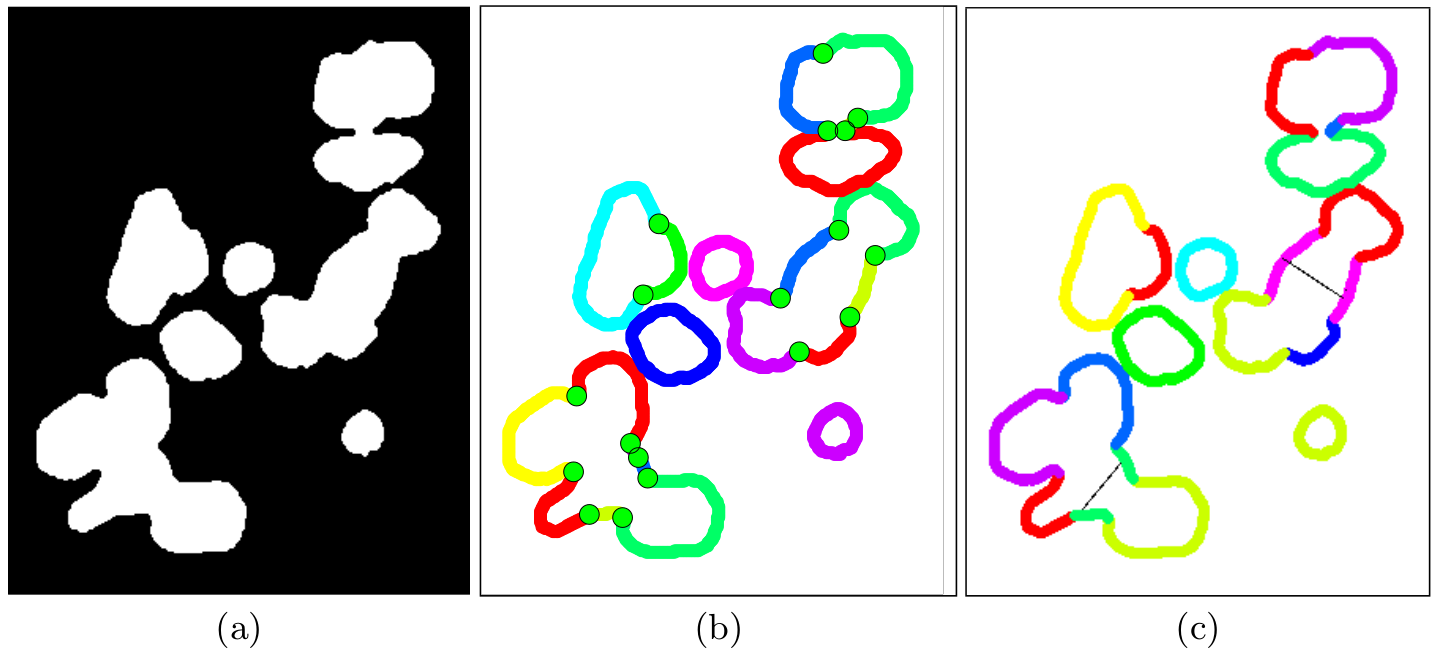
\includegraphics[width=\linewidth, scale=0.5]{segment-grouping.png}
  \caption{: Contour segmentation: 
    Segment grouping: 
    (a) Original image; 
    (b) Contour segmentation;
    (c) Segment grouping.~\cite{Zafari15}}
  \label{fig:Segment-grouping}
\end{figure}


To deal with the problem of a big amount of permutation researchers use different heuristics. Langlard~\emph{et al.}~\cite{LANGLARD2018} proposed the method that divides the cluster of overlapped elliptical objects to several sub-clusters. To do this, the authors search special split lines with the algorithm that was purposed by Farhan \emph{et al.}~\cite{farhan}. The visualization of the method is shown in Figure~\ref{fig:cluster-decomposition}.



\begin{figure}[htp]
    \centering {
        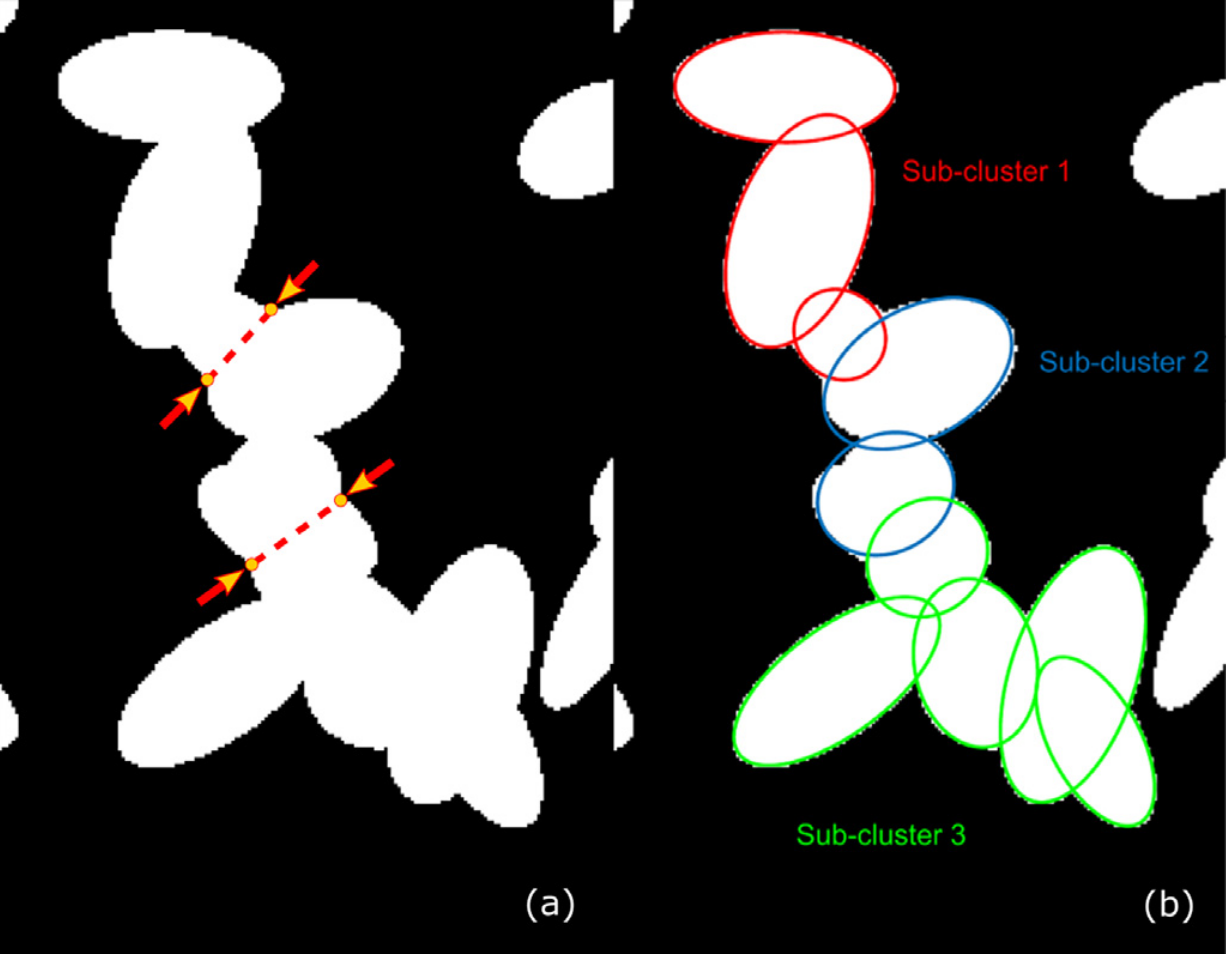
\includegraphics[width=100mm, scale=0.5]{subgrouping.png}
        \caption{Illustration of cluster decomposition and ellipse fitting: (a) Initial cluster and detected split; (b) Resulting sub-clusters and ellipse fitting.~\cite{LANGLARD2018}.}
        \label{fig:cluster-decomposition}
    }
\end{figure}

Zafari \emph{et al.} proposed two methods for segment grouping.  The first method~\cite{zafari-bb} limits search space by a rule that a distance between centers of segments is less than a predefined threshold value. The second method~\cite{zafari-bb} is based on the branch and bound optimization algorithm. The authors presented a new cost function that is a combination of two parts: 1) general part, which represents a convexity of the particle, and 2) specif part that represent the properties of objects with fixed elliptical shape. the specific part consist of two properties: symmetry and ellipticity. The full cost function formula~\cite{zafari-bb} is defined as:
\begin{equation}
    J = \alpha J_{concavity}+\beta J_{ellipticity} + \gamma J_{symmetry},
\end{equation}, where $\alpha,\beta,\gamma$ are weight coefficients.

\subsection{Contour Estimation}
\label{ContourEstimation}
The last step in the segmentation of overlapped object process is contour estimation. The most commonly used method for contour estimation is an ellipse fitting method. This method can be applied to many tasks in a segmentation of overlapped object area ~\cite{BE-FRS,Zhao2017,zafari-bb,LANGLARD2018}. This method uses the assumption that overlapped objects have an elliptical form. The Ellipse fitting approach is based on minimization the sum of distances between points and an ellipse. The definition of an ellipse equation is:
\begin{align}
    F(\textbf{a},(x,y)) &= a_0x^2 + a_1xy + a_2y^2 + a_3y + a_4y + a_5 = \textbf{a}^T \mathbf{x} = 0,
\end{align}
where $x$ and $y$ are the input points,$a_0...a_5$ are free parameters. Zhang~\emph{et al.}~\cite{acos_1} formulate the ellipse fitting problem as a  direct minimization of the equation 
\begin{equation}
    E = \sum_{i=1}^{n}d^2(\textbf{a}),
\end{equation}
where $d(\textbf{a}) = \sum_{i=1}^N{F(x_i, y_i)}$. This equation can be calculated by numerical methods.

The example of ellipse fitting is shown in Figure~\ref{fig:ellipse-fitting}.


\begin{figure}[htp]
    \centering {
        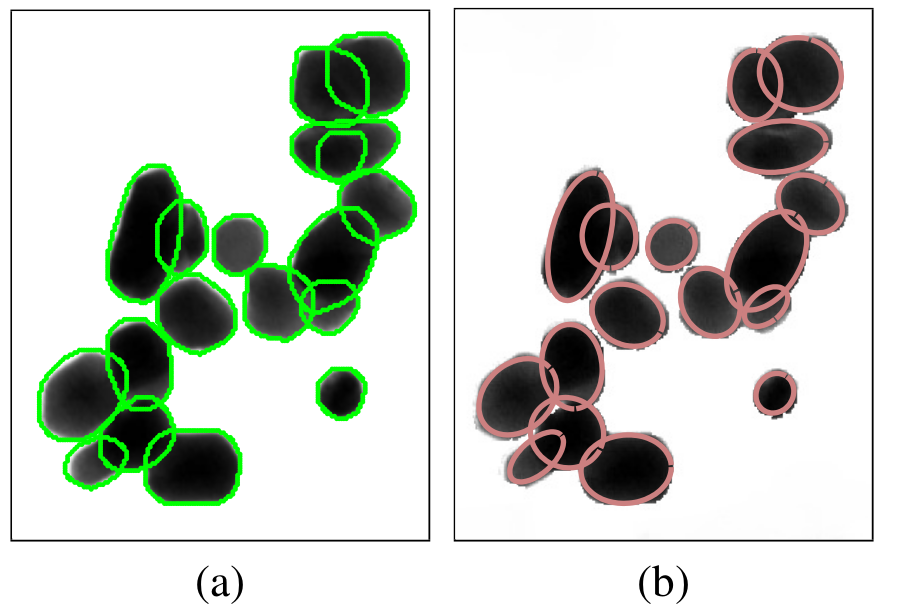
\includegraphics[width=\linewidth]{ellipse_fitting.png}
        \caption{Ellipse fitting method: (a) Manual fitting by a researcher; (b) Ellipse fitting.~\cite{BE-FRS}.}
        \label{fig:ellipse-fitting}
    }
\end{figure}


\section{PROPOSED FRAMEWORK}
\label{sec:proposed}

This section contains a description of a proposed framework for segmentation of convex overlapped objects.
The proposed framework is based on Branch and Boundaries framework~\cite{zafari-bb} with novel segment grouping function. The proposed framework implements the next pipeline (see Figure~\ref{fig:pipeline}:

\begin{enumerate}
    \item Image binarization and edge extraction.
    \item Concave points detection and contour segmentation.
    \item Contour segment grouping.
\end{enumerate}


\begin{figure}[ht]
    \centering
    \subfloat[][]{
            
\includegraphics[width=0.5\linewidth]{demo4.png}
            \label{subfig:grayim}
    }
    \subfloat[][]{
        
\includegraphics[width=0.5\linewidth]{SegmentsDemo.png}
        \label{subfig:segim}
    }
    
    \subfloat[][]{
        
\includegraphics[width=0.5\linewidth]{segmentationGP.png}
        \label{subfig:seggt}
    }
    
    \caption[]{
        \subref{subfig:grayim} A binary image;
        \subref{subfig:segim} a result of contour segmentation;
        \subref{subfig:seggt} a result of segment grouping.
    }
         
    \label{fig:pipeline}
\end{figure}

The novelty of the proposed method is in a segment grouping stage. However, the preceding stages have a significant effect on the success of the grouping. 


\subsection{Image binarization and edge extraction}

The image binarization and edge extraction stage is the most simple, but a very important part of the segmentation process. It consists of three stages: image binarization, smoothing and eroding the binary image, edge extraction.

\subsubsection{Image binarization}

Binarization of an original gray-scale image by an Otsu method~\cite{otsu}. This algorithm is a widely used algorithm that divides the image into two classes by an adaptive threshold. It uses the histogram of the image for a threshold searching process. It maximizes a "between class variance" of the segmented classes. Otsu proves that minimizing a "within class variance" is same as maximizing "between class variance" of the segmented classes. Furthermore, maximizing the "between class variance" is computationally less expensive than minimizing "within class variance".
   
\subsubsection{Smoothing and eroding the binary image}

Usually, the original images contain noise and sharp boundaries that must be smoothed. To deal with it the proposed framework applies morphological erosion~\cite{UECS} with a 3-pixel disk structuring element. This smooths the boundaries and reduces a noise that can be detected as small particles.
 
\subsubsection{Edge extraction}

Edge extraction is performed by a Canny detector~\cite{Canny}. The algorithm of this detector the has following steps.

The first step of the algorithm is smoothing. During this step, the image is smoothed and the regions of the picture with high first spatial derivatives are highlighted.


The next step is a searching of gradients. The detector marks the boundaries in the places where the gradient is a local maximum. To find it, the Canny detector uses four filters, which search gradients of different directions. After that, the detector reduces all non-local maximum gradients.

The final step is an edge tracking. The tracking process is controlled by two thresholds: $T1$ and $T2$, where $T1 > T2$. Tracking can only start at a point on an edge greater than $T1$. Tracking then proceeds in both ways out from that point until the height of the edge drops below $T2$. This hysteresis helps to guarantee that noisy edges are not split up into various edge pieces.

\subsection{Concave points detection and segmentation}

For concave point extraction a modified curvature scale space (CSS) method~\cite{CSS} was selected. 

Firstly, the method calculates for each border point, curvature value~\cite{CSS} and selects the points, which are local extrema for curvature values.  

The output points, so-called \textit{dominant points}, lie on both convex and concave regions of the object boundaries. To choose just concave points, the method filtrates points with the following criteria. A dominant point is a concave point if the line, connecting left and right neighbors of this point, does not reside inside the object. 

Finally, the framework split particles contours into segment edges by concave points.
%TODO: image

\subsection{Segment grouping}

Segment grouping method is a part of segmentation framework, that merge segments, which belongs to one object. Segment grouping stage is a modification of the original segment groping stage in Branch and Boundaries framework~\cite{zafari-bb}.  Segment grouping could be divided into two steps: 1) a preprocessing step, and 2) a branch and boundaries algorithm step.

\subsubsection{Preprocessing} 
During preprocessing step, the framework creates so-called \textit{grouping matrix}, a special concavity matrix of all segments, that show can two segments be, hypothetically, united to one group, or not. To estimate this ability, two heuristics are used: adjacency and attainability.

Adjacency is a simple heuristic that is based on an idea that two neighbor segment cannot be grouped because in another way there could not be a concave point between them  (see Fig.~\ref{fig:neib}). To determinate that two segments are neighbors, the segment grouping method check that Euclidean distance between ends of the segment is less than 4 pixels.

Attainability is more complicated heuristic which validates that two segments can be united to one polygon, and this polygon does not intersect other segments (see Fig.~\ref{fig:intersection}). The segment grouping method performs this test in the way, which is described in Algorithm~\ref{alg:HeuristicIntersection}.


\begin{algorithm} [H]
    \SetAlgoLined
    \KwData{segments}
    \KwResult{attainability matrix}
    Represent all segments as sequences of points\;
    Create shapes for each pair of segments\;
    \ForAll{shape in shapes}{
        Test that there are not any points inside shape, except the points which belong to segments that formed the shape\;
    }
    
\caption{Attainability test.}\label{alg:HeuristicIntersection}
\end{algorithm}



\begin{figure}[htp]
    \centering {
        
\includegraphics[width=0.5\linewidth]{neibour.png}
        \caption{A pair of neighbour segments (red and blue).}
        \label{fig:neib}
    }
\end{figure}


\begin{figure}[htp]
    \centering {
        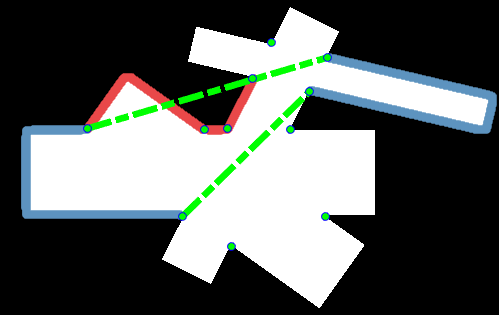
\includegraphics[width=0.5\linewidth]{intersection.png}
        \caption{A pair of segment, which shape is intersected other segments (blue is a pair of segments, red is intersected segments, green points is concave points, greed lines are invisible lines of the pair shape).}
        \label{fig:intersection}
    }
\end{figure}


\subsubsection{Branch and Bound algorithm}
The segment grouping task can be represented as a combination problem of optimal separation of N objects to M groups. However, this is an NP-hard problem~\cite{bubble} and cannot be solved by brute force algorithms. One of the most commonly used methods to find a solution for NP-hard problems is a branch and bound (BB) algorithm~\cite{bubble}.  BB is efficient for an optimization problem since it avoids exhaustive enumeration using the value of the current optimal solution
and defining bounds for the function to be optimized. The BB algorithm is used as a segment grouping algorithm in the original BB framework~\cite{zafari-bb}. In this thesis, a novel cost function for the BB algorithm is proposed.

The BB algorithm can be easily demonstrated on the example, that shown in Figure~\ref{fig:seg-bb}. Let $S=\{S_1,S_2,S_3,S_4\}$ is set of segments and $J$ is a cost function. To decrease the number of all segment group combinations, let say that grouping candidates $\{S_1,S_2\}$ and $\{S_2,S_1\}$ are the candidates because the groups differ if they contain different segments. 


\begin{figure}[htp]
    \centering {
        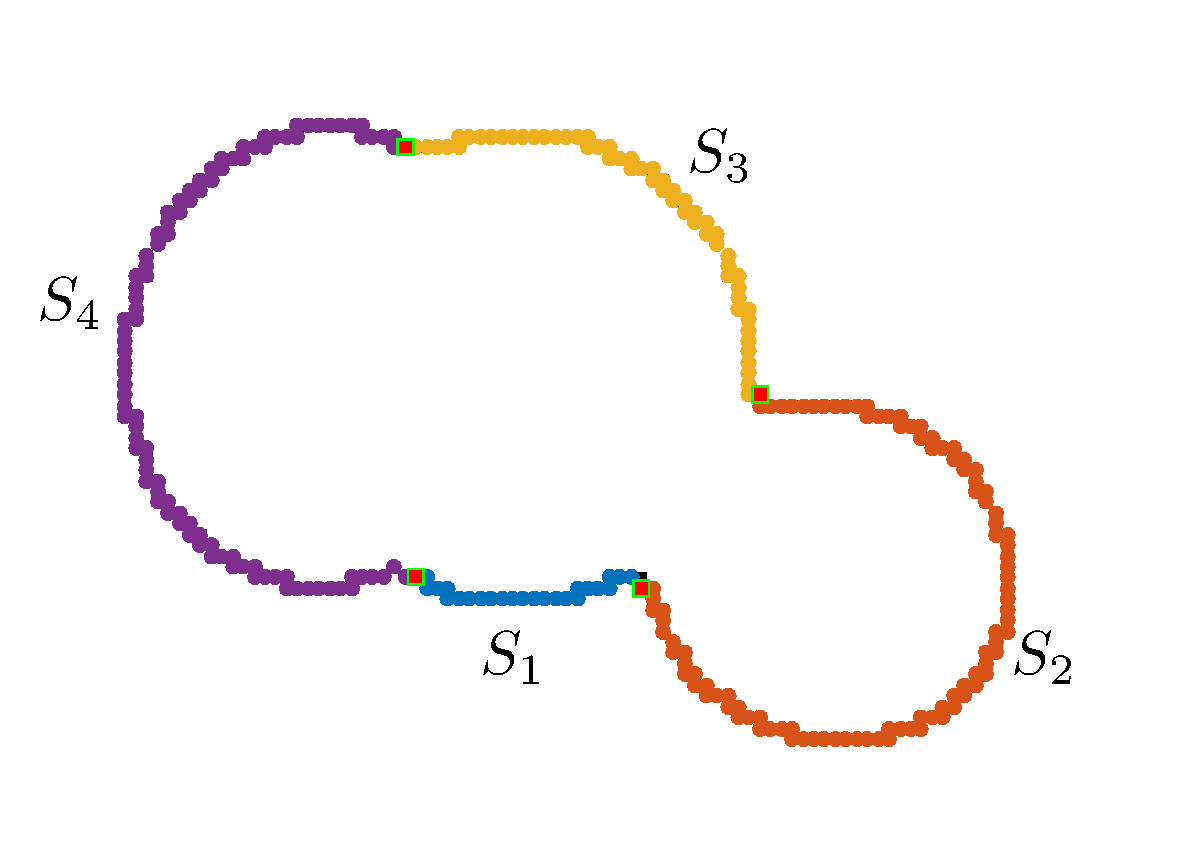
\includegraphics[width=50mm, scale=0.5]{segments.pdf}
        \caption{An instance of contour segments.~\cite{zafari-bb}}
        \label{fig:seg-bb}
    }
\end{figure}

In the Figure~\ref{fig:full-bb} the search tree with all possible segment groups are shown.  The initial state represents grouping candidates which contain just one segment. Each n level represents all possible grouping candidates that contain n segments.   




\begin{figure}[htp]
    \centering {
        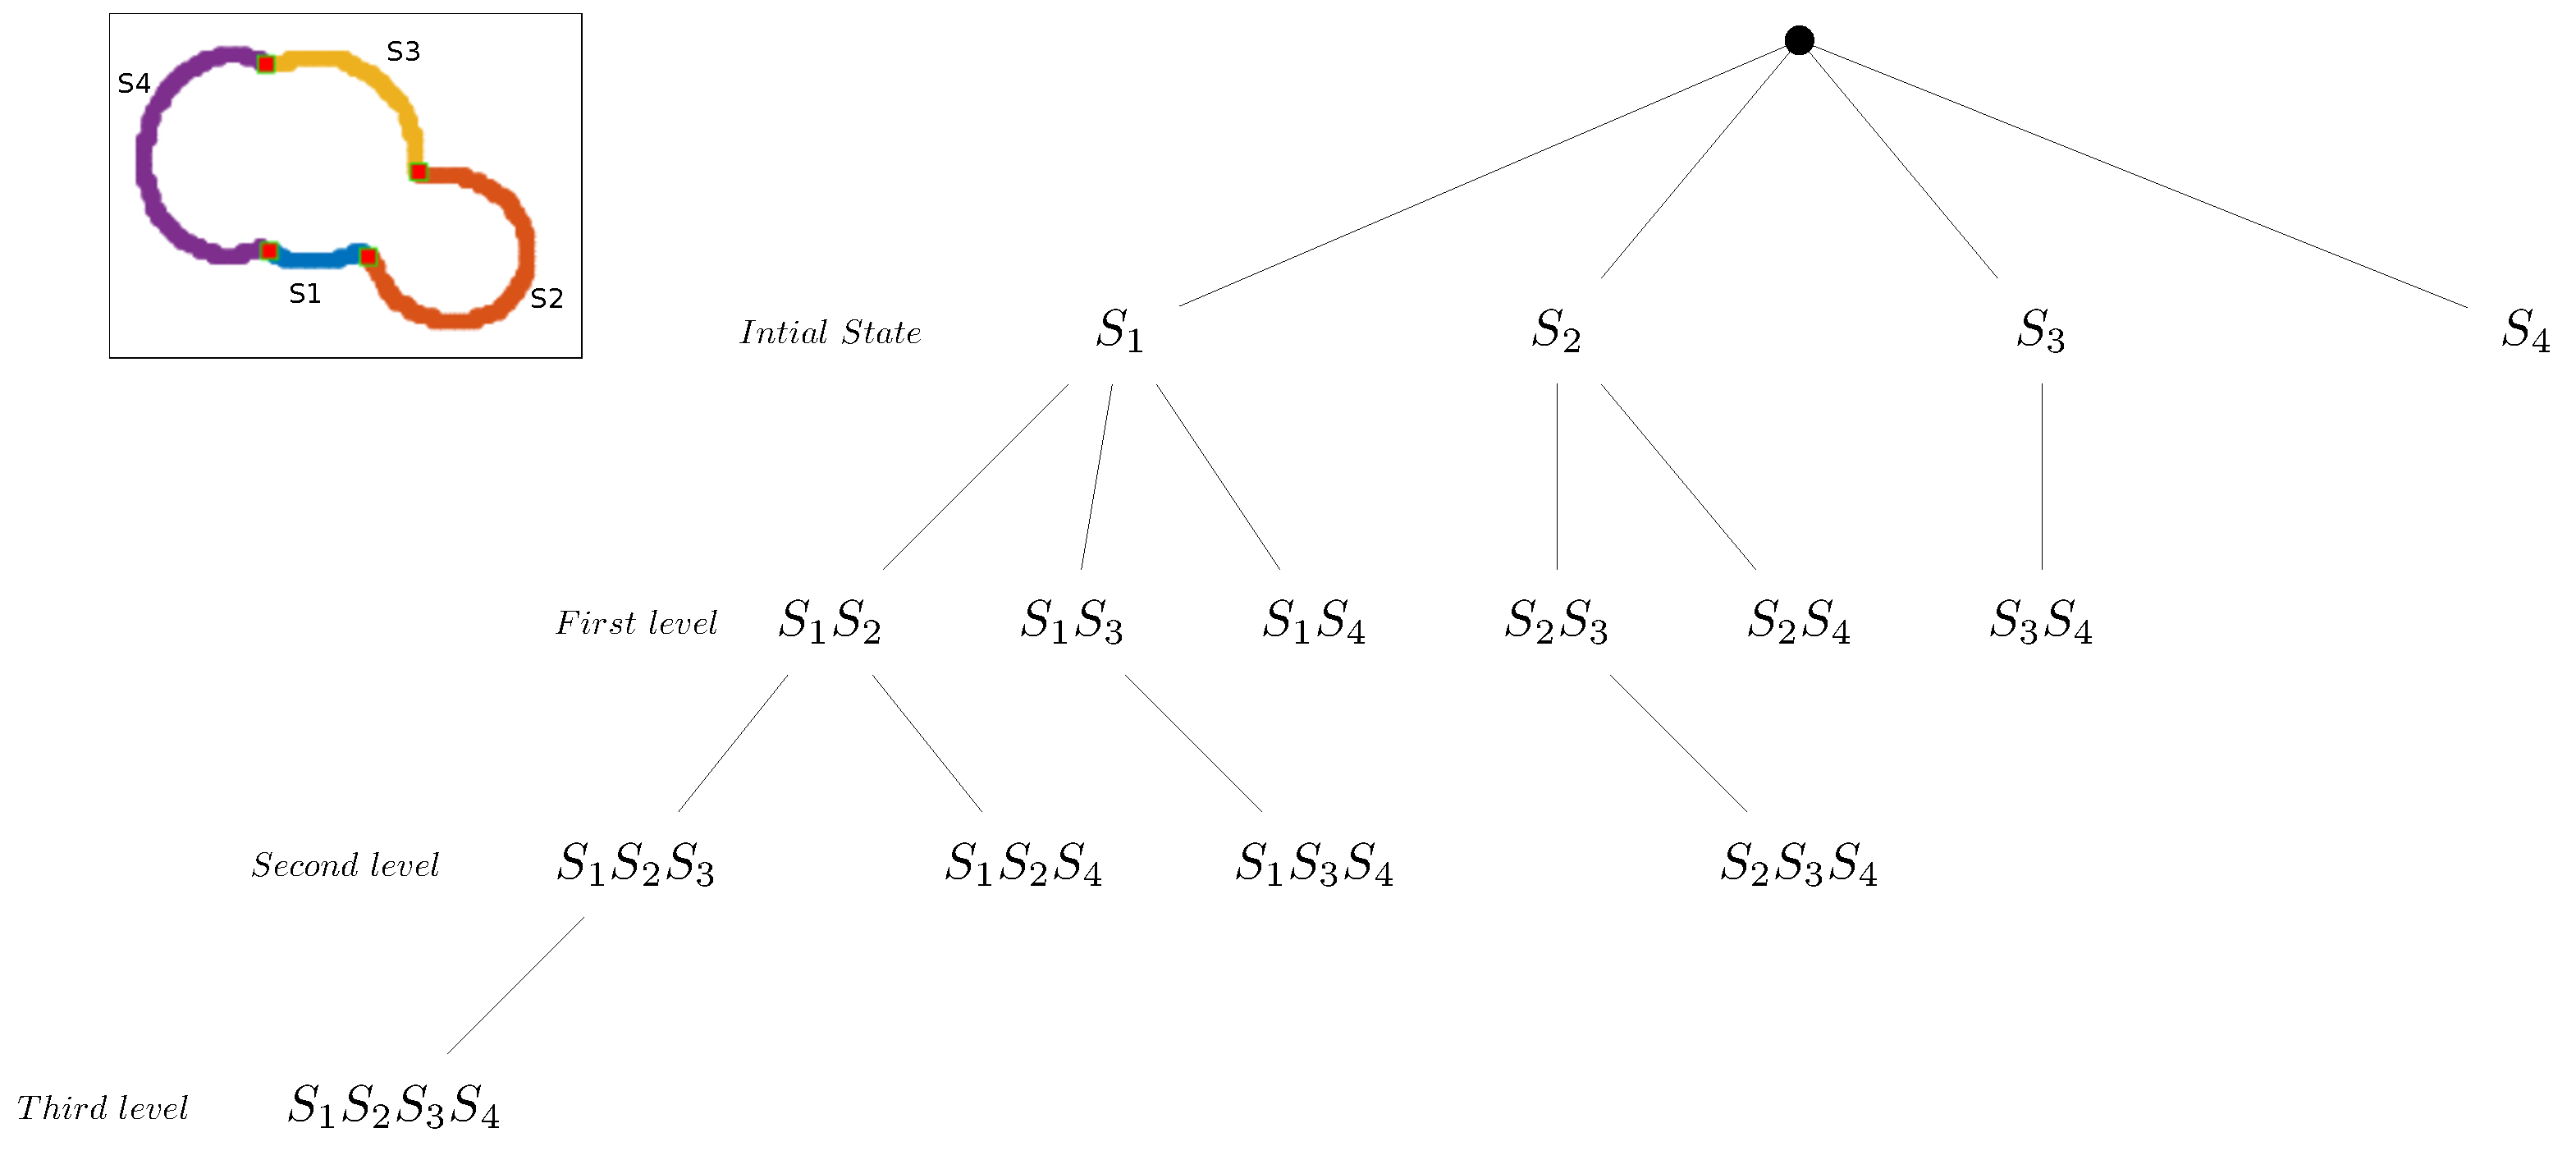
\includegraphics[width=\linewidth]{bb_search_tree_all_2.pdf}
        \caption{The visualization of the full searching tree.~\cite{zafari-bb}}
        \label{fig:full-bb}
    }
\end{figure}



The nodes of the search tree are exploded by depth-first search algorithm~\cite{zafari-bb}. The optimal grouping is a node with the minimal cost function. To reduce the number of grouping candidates nodes the algorithm uses the following test. Let $B = J(\{S_1,S_2\})$ is a cost function value for a grouping candidate $\{s_1\}$.  Let $\{s_1,s_2\}$ is a children node of $\{S_1\}$. If the $J(\{S_1,S_2\})>B$ then the BB algorithm will not extend the tree for $\{s_1,s_2\}$ node, because the child is worse then the parent.

The result of the BB algorithm for $S$ is shown in Figure~\ref{fig:bb}. Is it can be seen in the Figure the cost value $J(S_1,S_2)>B$, so the algorithm is not extend the search tree in this way, but $J(s_1,s_3)<B$, so the BB algorithm adds child node $\{S_1,S_2,S_3\}$ into the searching tree. The result of segment grouping for $S$ are following groups: $\{S_1,S_2\}$, $\{S_2\}$, $\{S_4\}$. 


\begin{figure}[htp]
    \centering {
        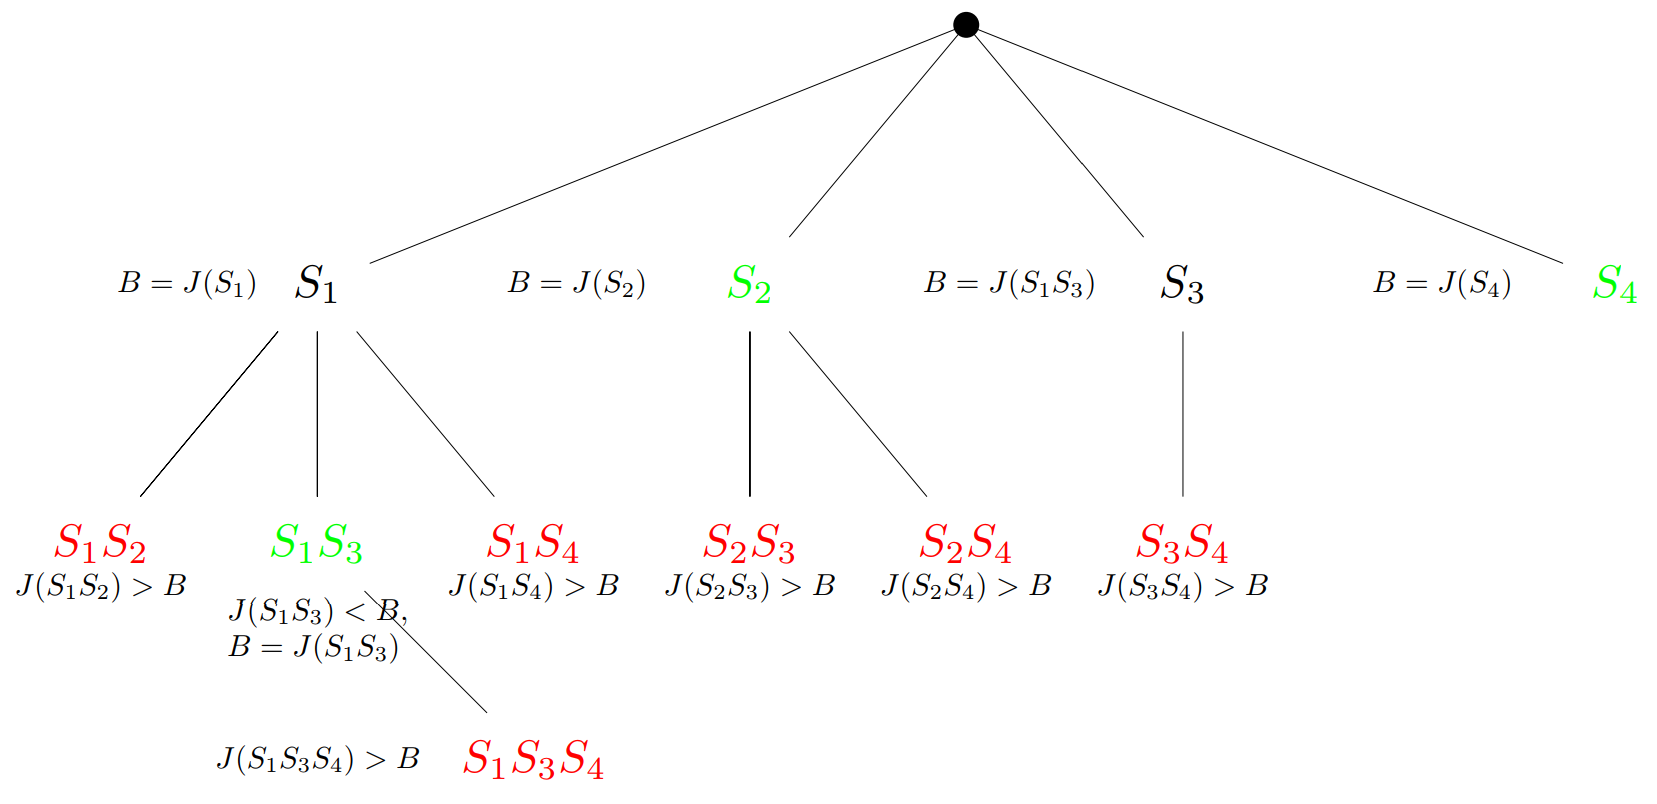
\includegraphics[width=\linewidth]{bb.png}
        \caption{An example of a result of a BB algorithm work.~\cite{zafari-bb}}
        \label{fig:bb}
    }
\end{figure}

\subsubsection{Cost function for BB algorithm}

The key part of the BB algorithm is a cost function. A cost function represents the quality of grouping and makes possible to compare two segmentation candidates. To estimate the cost function, in~\cite{zafari-bb}, it was assumed that particles have an elliptical form and a cost function was created based on symmetry, convexity, and ellipticity.

In this thesis, a novel cost function was developed. The cost function is based on a hypothesis that objects have a convex form and the shape is similar to one of the next type of shapes: ellipse, quadrilateral, or triangle. The grouping cost calculation algorithm consists of several parts and is shown in Algorithm~\ref{alg:CostFunction}.

Firstly, the segments in a groping candidate must be adjacent to each other in grouping matrix. If at least one pair of segments is not adjacent, the grouping cost is set to infinity.

The second step is a rearrangement of grouping candidate segments. It is a necessary operation because the convexity checking function requires segments sorting by a clockwise order. The algorithm~\ref{alg:sort} describes the main steps of sorting. The complexity of the sort algorithm is $O(n^2)$.


\begin{algorithm} [H]
    \SetAlgoLined
    \KwData{input segments}
    \KwResult{sorted segments}
    let n is a number of segments\;
    let S is is an empty array with sorted segments\;
    \For{i = 1..n}{
        add to S a segment from the input segments which maximize the area\\
        of the sorted segments shape\;
    }
    \Return{S}
\caption{Cost function.}\label{alg:sort}
\end{algorithm}

The next step of cost function calculating is shape fitting. For this framework, the type of figures was limited by ellipse, quadrilateral, and triangle, as the most common types. To determinate the similarity of a segment group to one to the shape are used the following trick. The framework calculates the area ($A_{segments}$) of the segment group polygon. Next, the segments are represented as a cloud of points. For the cloud of points, the algorithm builds an ellipse, a quadrilateral, and a triangle, which cover the points and have a minimal area. To build shapes with the minimal area a suite of minimal bounding~\cite{suite} objects were used. 

To estimate an area of the minimal bounding triangle ($A_{triangle}$) is used the following algorithm: 1) for each edge of the shape was build a triangle that has this edge in the base and covers all points, 2) selected a triangle with minimal area.

The algorithm which determinates a minimal bounding quadrilateral ($A_{quadrilateral}$) the following: 1) sort all edges in counter-clockwise order 2) find the combination of 4 edges, which form a  quadrilateral with minimal area.

The minimal area of a covering ellipse ($A_{ellipse}$) is calculated by the way that was described by minimization the sum of distances between points and an ellipse. The paragraph~\ref{ContourEstimation} has a more detailed explanation.

The similarity ($S$) of the segments group is calculated as: 
\begin{equation}
    S = \frac{\min(A_{triangle},A_{ellipse},A_{quadrilateral})}{A_{segments}}.
    \label{eq:simularity cost}
\end{equation}

The final step is a groping cost calculation.  The grouping criteria should encourage the big amount of segment in a group. It can be done by simply dividing the result of previous steps by the count of segments ($N$). So the final grouping criteria are:
\begin{equation}
    J = \frac{S}{N}.
    \label{eq:fullCost}
\end{equation}



\begin{algorithm} [H]
    \SetAlgoLined
    \KwData{segments, grouping matrix}
    \KwResult{cost}
    \If {one or more pair of segment is not adjacent in grouping matrix} {
     \Return {$\infty$ }
    }
    sort segments clockwise\;
    check segments group convexity\;
    \If {group is not convex} {
        \Return {$\infty$ }
    }
    calculate similarity by Eq.~\ref{eq:simularity cost}\;
    calculate grouping cost by Eq.~\ref{eq:fullCost}\;
    \Return{grouping cost}
\caption{Cost function.}\label{alg:CostFunction}
\end{algorithm}

\section{EXPERIMENTS}
\label{sec:experiments}

\subsection{Data}
For validation of the proposed method, two types of data were used: real data and synthetic data.
 
The synthetic dataset (see Figure~\ref{fig:imex}(a))consists of images with 25 overlapping
objects of three different types: ellipses, triangles, and quadrilateral. All objects were uniformly randomly translated, scaled and rotated. All generated images have a size of 700x500 pixels, and a maximum rate of the overlapping area is 40\%. The dataset consists of 12 generated images. Every image was generated with a ground truth text file which contains boundaries of the figures.

The real dataset contains images of nanoparticles, captured
using transmission electron microscopy (see Figure~\ref{fig:imex}(b)). In result, the dataset contains 11 images of 4008x2672 pixels. Approximately 200 particles were marked manually in each image by a specialist. The ground truth consists of manually drawn contour segments and contour segments groups. 

The examples of images is shown in the appendix Figures~\ref{fig:realdata} and~\ref{fig:syntheticdata}.

\begin{figure}[ht]
    \centering
    \subfloat[][]{
            
\includegraphics[width=0.5\linewidth,height=5cm]{img001.png}
            \label{subfig:syn_image}
    }
    \subfloat[][]{
        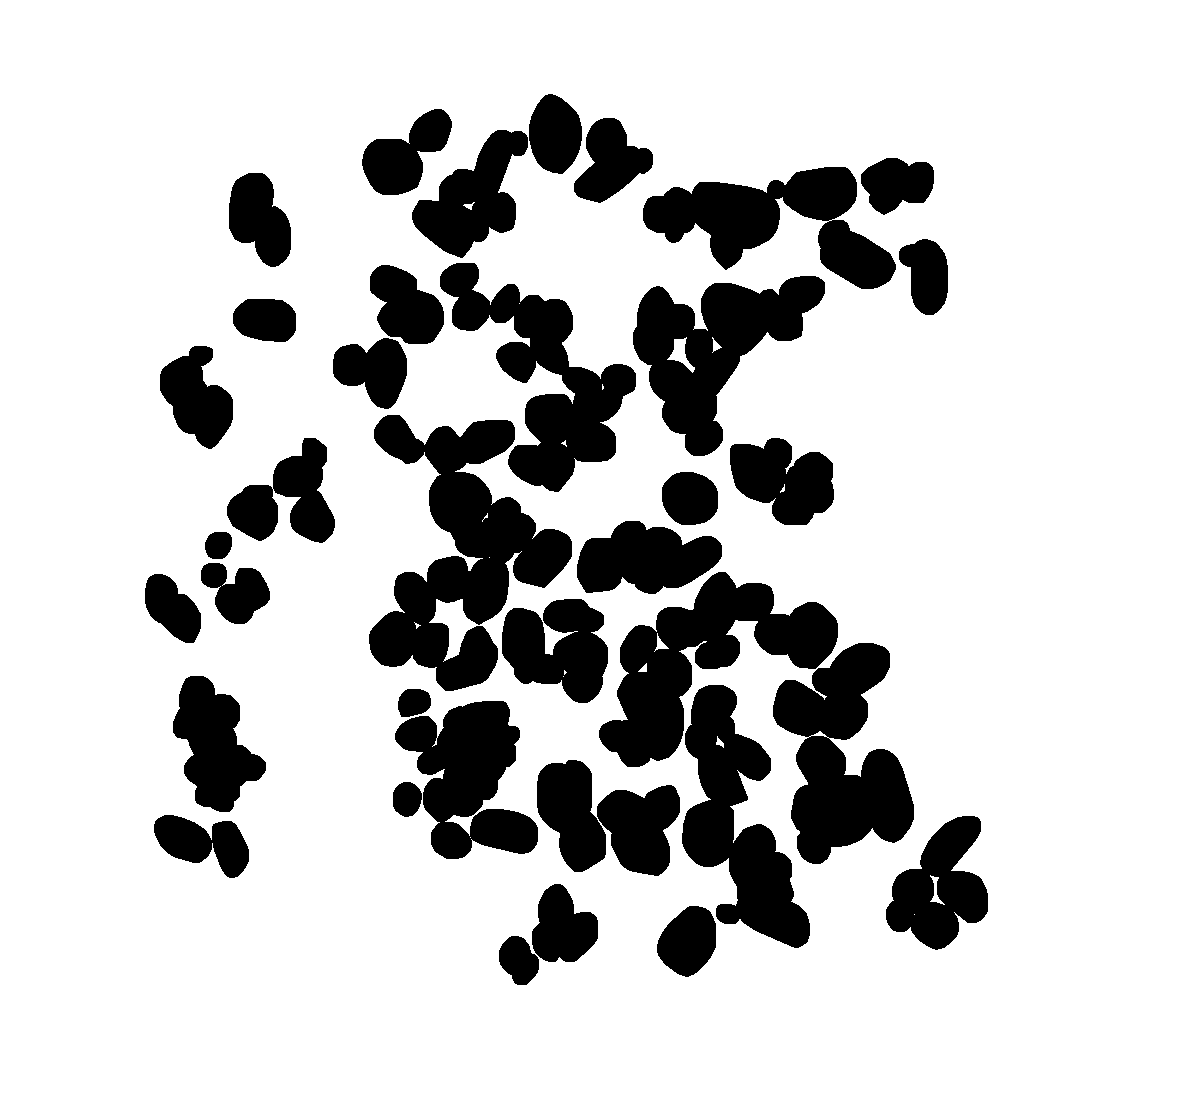
\includegraphics[width=0.5\linewidth, height=5cm]{realimage02e.png}
        \label{subfig:real_image}
    }
    
    \caption[]{
        Examples of data:
        \subref{subfig:syn_image} a synthetic image;
        \subref{subfig:real_image} a real image.
    }
         
        \label{fig:imex}
\end{figure}

\subsection{Evaluation criteria}
A segment grouping task can be evaluated as a clusterization problem where the count of predicted classes may differ from the ground truth. Ground truth is a result of segment grouping that was gotten from real shapes of particles. One of the best metrics of clusterization is Maximum-Match-Measure (MMM)~\cite{mm-estimate}. This metric was selected for several reasons. Firstly, this metric admits the difference between a number of real groups and predicted. Secondly, this metric is tolerant to the different labels for the same segments in the predicted and ground truth contour segment grouping results. This measure tries to find an optimal matching between the predicted results and the ground truth segment groups.

The algorithm of MMM can be shown by an example. Let the predicted segment groups for the segments in Figure~\ref{fig:seg-bb} are $\{S_1,S_3,S_4\}$ and $\{S_2\}$, the ground truth segment groups are $\{S_1,S_3\}$,$\{S_2\}$,$\{S_4\}$.

The similarity matrix are built as:
\begin{equation}
MM_{origin} = 
        \begin{bmatrix}
            2& 0 \\
            0& 1 \\
            1& 0
        \end{bmatrix}.
    \end{equation}
It means that: the predicted group 1 has 2 elements from the expected group 1, 0 from the expected group 2, and 1 from the expected group 3, and so on.
After that, the maximum-match algorithm tries to find the 2x2 matrix with maximum trace (diagonal sum). In the case of the example, it is

\begin{equation}
MM_{reduced} = 
        \begin{bmatrix}
            2& 0\\
            0& 1
        \end{bmatrix}.
    \end{equation}
The result of MMM is the sum of diagonal elements devided by the sum of all elements of $MM_{origin}$. For this example, it is 
\begin{equation}
        MMM = \frac{2+1}{4}=0.75.
\end{equation}



\subsection{Results}

The proposed segment grouping method was compared with original branch and boundaries segment grouping method proposed in~\cite{zafari-bb}. The results for synthetic and real data are shown in Tables~\ref{tab:syndata} and~\ref{tab:realdata}.


\begin{table}[hpt]
\begin{center}
\caption{The result of validation comparing for synthetic data.\label{tab:syndata}}
\begin{tabular}{ |c||c|c|  }
 \hline
 Number & Proposed method & Zafari BB~\cite{zafari-bb}\\
 \hline
 1   &  0.85&  0.57\\
 2   &  0.74&  0.56\\
 3   &  0.73&  0.5\\
 4   &  0.75&  0.55\\
 5   &  0.71&  0.53\\
 6   &  0.90&  0.52\\
 7   &  0.81&  0.72\\
 8   &  0.85&  0.78\\
 9   &  0.80&  0.55\\
 10  &  0.71&  0.52\\
 11  &  0.93&  0.73\\
 12  &  0.83&  0.65\\
 \hline
 \textbf{\textit{Mean}} & 0.80 & 0.65 \\
 \hline
\end{tabular}
\end{center}
\end{table}


\begin{table}[hpt]
\begin{center}
\caption{The result of validation comparing for real data.\label{tab:realdata}}
\begin{tabular}{ |c||c|c|  }

 \hline
 Number & Proposed method & Zafari BB~\cite{zafari-bb}\\
 \hline
 1   &  0.62&  0.78\\
 2   &  0.59&  0.74\\
 3   &  0.57&  0.79\\
 4   &  0.53&  0.64\\
 5   &  0.65&  0.59\\
 6   &  0.77&  0.74\\
 7   &  0.70&  0.70\\
 8   &  0.66&  0.72\\
 9   &  0.65&  0.80\\
 10  &  0.56&  0.74\\
 11  &  0.51&  0.72\\
 \hline
 \textbf{\textit{Mean}} & 0.62 & 0.71\\
 \hline
\end{tabular}
\end{center}
\end{table}

From the result with the synthetic dataset (Table~\ref{tab:syndata}) it can be seen that
the proposed algorithm shows the best results. This is because the original BB method have an assumption that objects have approximately elliptical shape. The proposed method is developed to recognize all types of shapes in the synthetic dataset.


The results on the nanoparticles dataset (Table~\ref{tab:realdata}) show different results. The proposed algorithm worse than original BB algorithm. It is connected with two reasons. The first reason is that the real data contain a lot of of particles, and some have not convex shape, what is a critical for proposed algorithm. The second reason is that all particles are predominantly symmetrical and have elliptical form. The proposed algorithm does not take into account the symmetry of objects in contrast to the original algorithm.

The result of segment grouping of the proposed method and the original BB algorithm is shown in Figure~\ref{fig:comparing}.

\begin{figure}[ht]
    \centering
    \subfloat[][]{
            
\includegraphics[width=0.5\linewidth]{segmentationGP.png}
            \label{subfig:proposed}
    }
    \subfloat[][]{
        
\includegraphics[width=0.5\linewidth]{demoBB.png}
        \label{subfig:bb}
    }
    
    \subfloat[][]{
        
\includegraphics[width=0.5\linewidth]{SegmentsDemo.png}
        \label{subfig:segments}
    }
    
    \caption[]{
        \subref{subfig:proposed} A result of segmentation of the proposed segment grouping method;
        \subref{subfig:bb} a result of segmentation of the original BB method~\cite{zafari-bb};
        \subref{subfig:segments} a result of segmentation.
    }
         
    \label{fig:comparing}
\end{figure}
\section{DISCUSSION}
\label{sec:discussion}

\subsection{Current study}


In this work, a new segmentation framework with a novel segment grouping method. The segmentation framework consists of the following parts: image preprocessing, concave points detection and segmentation, and segment grouping.

The image preprocessing stage prepares an image for concave points extraction and segmentation. This step includes binarization of an image by an Otsu method~\cite{otsu}, smoothing and reducing noise. Finally, there is an extraction of edges on the image by a Canny detector~\cite{Canny}. 

the concave points detection and segmentation stage are performed in two steps. Firstly, the framework extracts concave points by CSS algorithm~\cite{CSS}. Furthermore, the framework split particles contours into segment edges by concave points. 

The segment grouping stage consists of two parts: a preprocessing and a branch and bound optimization. During the first part of this stage, the framework for every pair of segments checks two heuristics: if there is at least one segment between these segments, and if the segments are neighbors to test the segments can be in one segment group. The main part of this stage is the Branch and Bound algorithm. The grouping task is an NP-hard~\cite{zafari-bb} problem and BB is one of the methods that can reduce the computational time. The implementation of the BB algorithm was based on~\cite{zafari-bb} with the proposed cost function.

A cost function is the most important part of the BB algorithm because it makes possible to estimate the quality of grouping. The cost function is based on the following assumptions: similarity to one of the predefined shapes, convexity.

The synthetic dataset consists of 12 images. Each image contains 25 overlapping objects of three different types: ellipses, triangles, and quadrilateral. The real dataset consists of 11 images of nanoparticles, captured
using transmission electron microscopy.


As an evaluating criterion Maximum-Match-Measure criteria were selected.  This criteria searches maximal matching between ground truth and predicted segment grouping results and is tolerant to a different number of predicted and ground truth segment groups. The proposed method was compared with the original Branch and Bound~\cite{zafari-bb} algorithm.

The result of experiments showed that proposed method outperforms existed solution on the synthetic data, but shows the worse result with the real data.

\subsection{Future work}

The segment grouping function proposed in thesis paper can be improved by several ways.

The first way is to add symmetry calculation in the cost function. It is connected with an observation that real particles usually have a symmetrical shape. 

The second way is to extend the list of recognized types of shapes. For instance, it can be a good idea, for example, to add a hexagon, a semicircle, etc. An extended list of shapes can improve the performance of the algorithm.


\section{CONCLUSION}
\label{sec:conclusion}

In this work methods for segment grouping were studied and a new segment grouping framework was proposed. A survey of existing segmentation methods was made in order to understand which methods can be used for the tasks of segmentation and segment grouping. There are two main approaches for segmentation. The one is based on seed-points detection and the other is based on concave points extraction. The proposed framework is based on the original BB algorithm~\cite{zafari-bb} with a proposed cost function. This cost function based on shapes fitting and allows users to group segments of convex objects with ellipse, quadrilateral and triangle forms. 

The proposed cost function was compared with original BB cost function~\cite{zafari-bb} on the real and the synthetic data. The results of the experiments showed that the proposed cost function outperforms the original cost function on the synthetic data.

\clearpage

% Bibliography
%
%% This must be here, not in preamble, if you want it to work
\addcontentsline{toc}{section}{REFERENCES}
\bibliography{resources/thesis}



%% ----------------------- APPENDICES ------------------------------

\appendix
 
\section{Examples of data images}
\label{appendix:graph}


\begin{figure}[ht]
    \centering
    \subfloat[][]{
        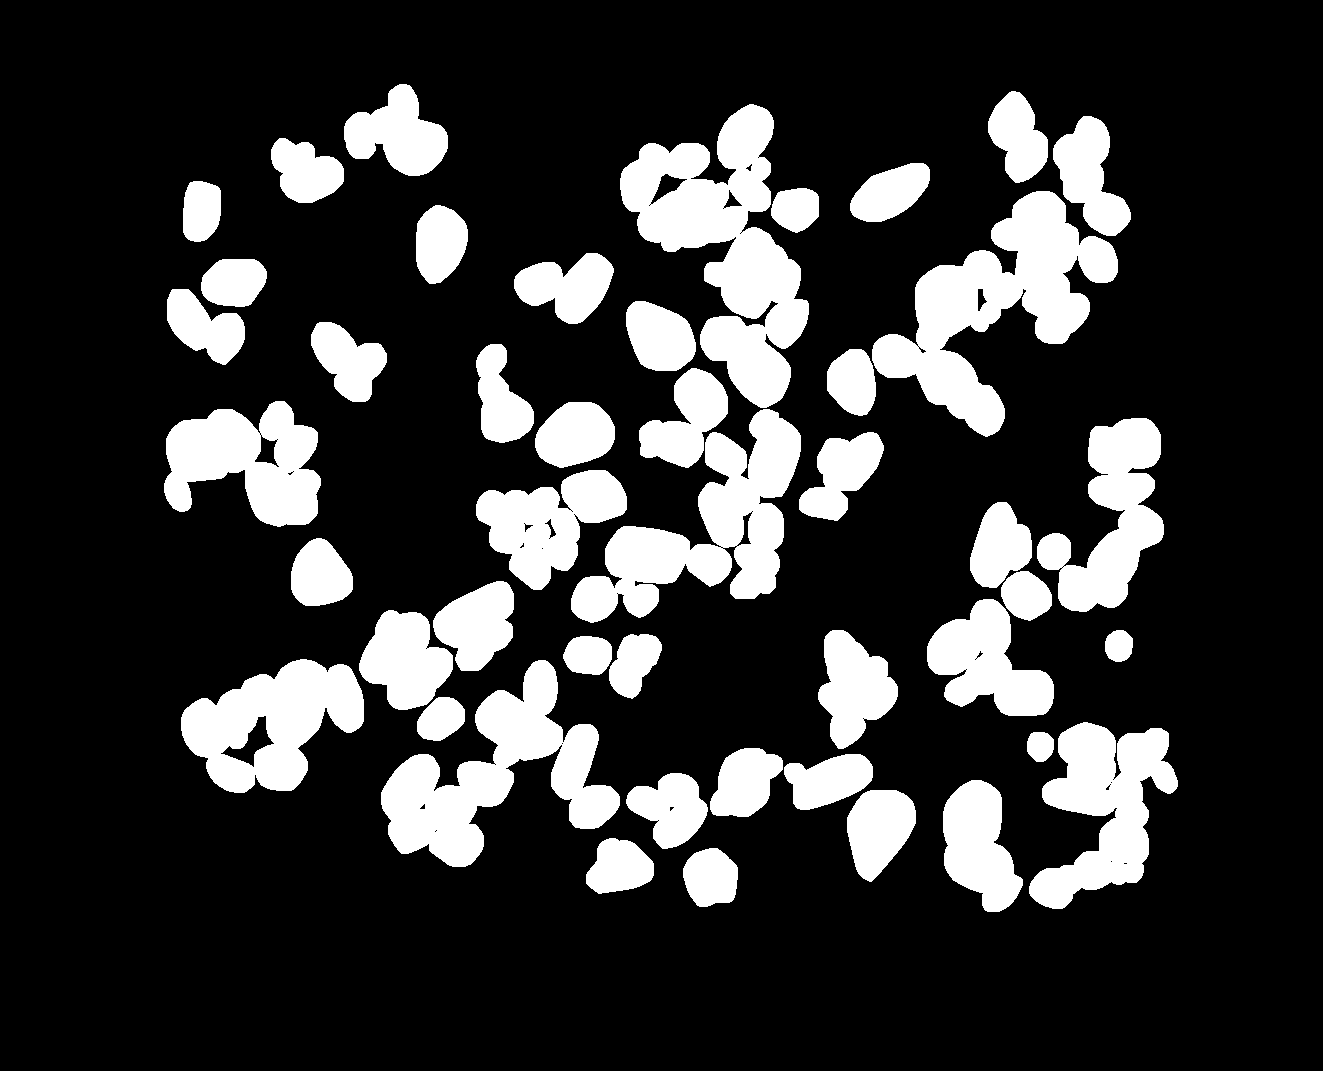
\includegraphics[width=0.5\linewidth]{realimage01.png}
    }
    \subfloat[][]{
            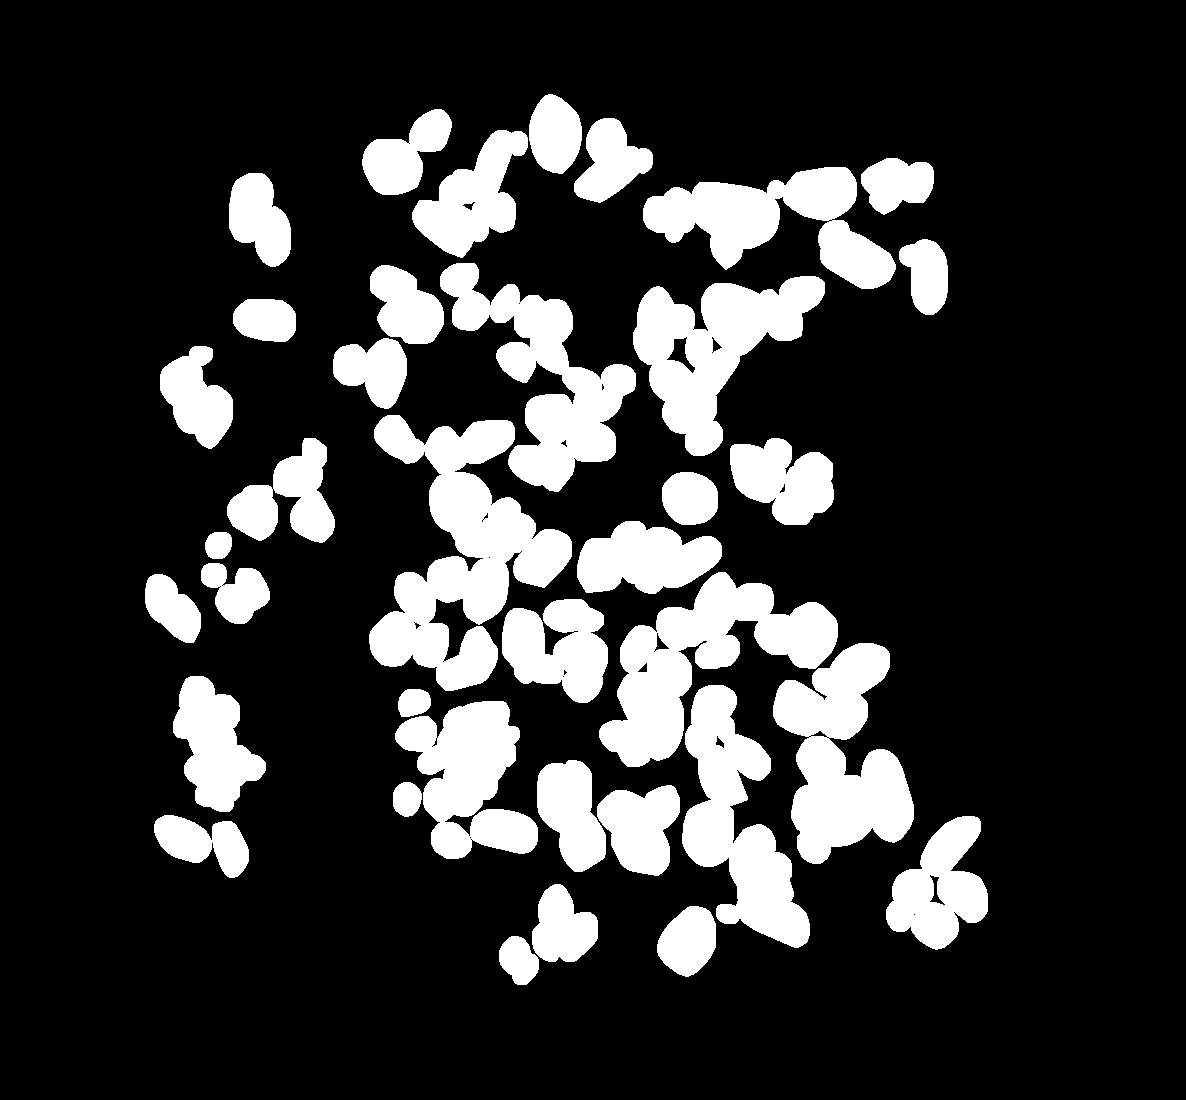
\includegraphics[width=0.5\linewidth]{realimage02.png}
    }
    \\
    \subfloat[][]{
            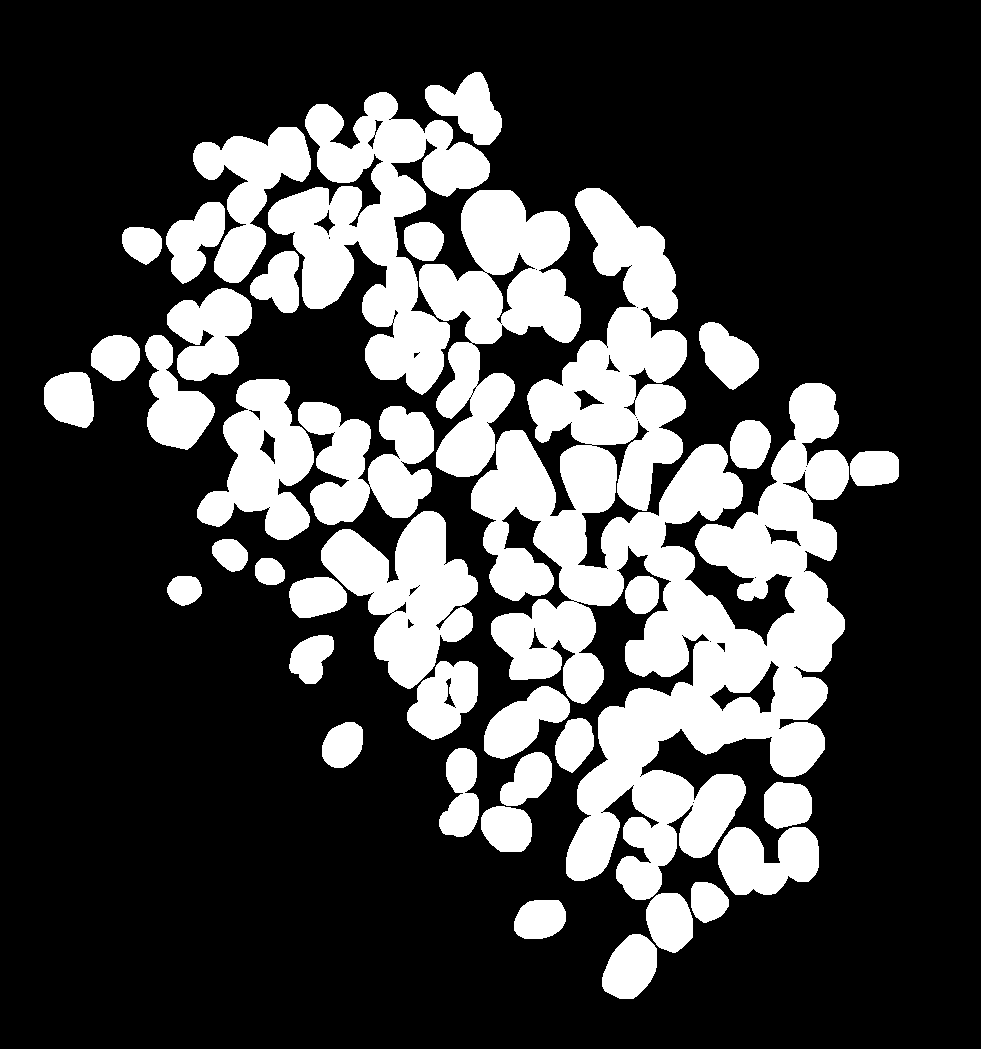
\includegraphics[width=0.5\linewidth]{realimage05.png}
    }
    \subfloat[][]{
            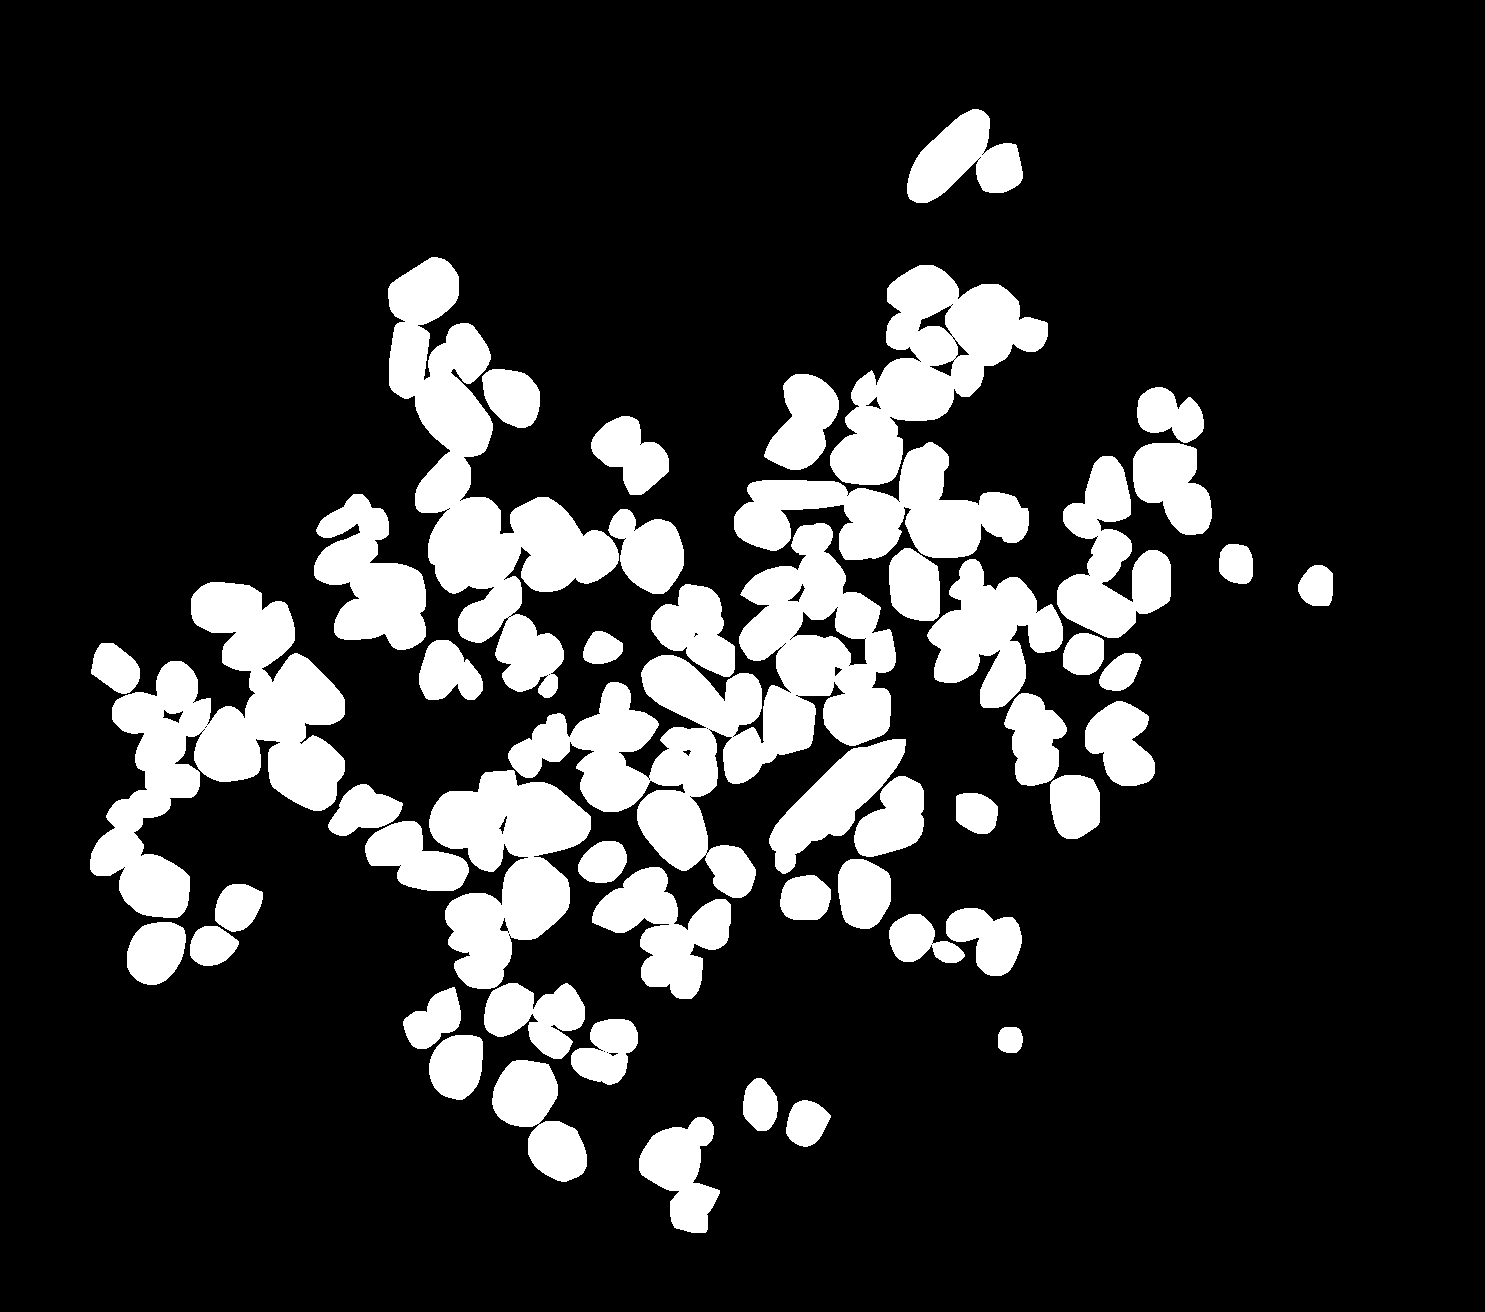
\includegraphics[width=0.5\linewidth]{realimage07.png}
    }
    \\
    \subfloat[][]{
            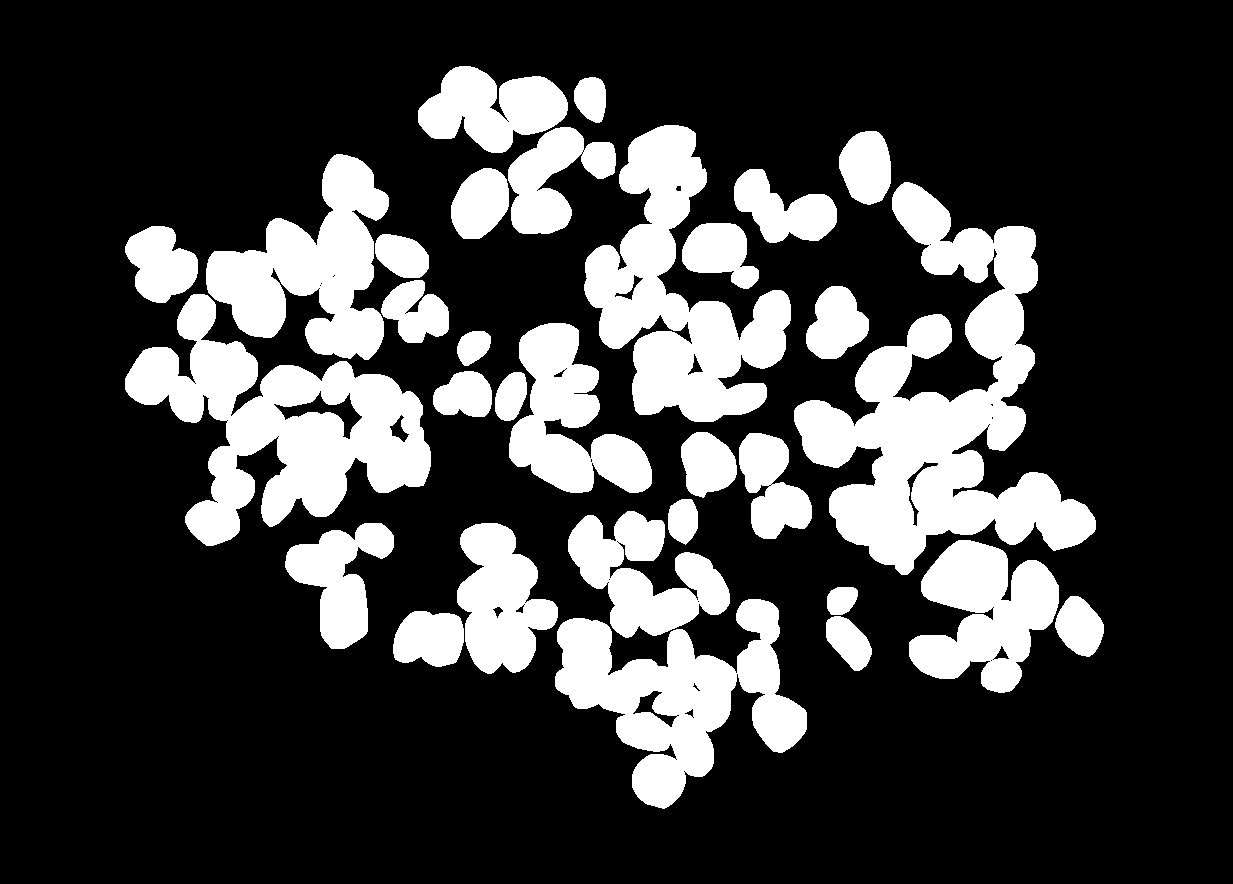
\includegraphics[width=0.5\linewidth]{realimage03.png}
    }  
    \subfloat[][]{
            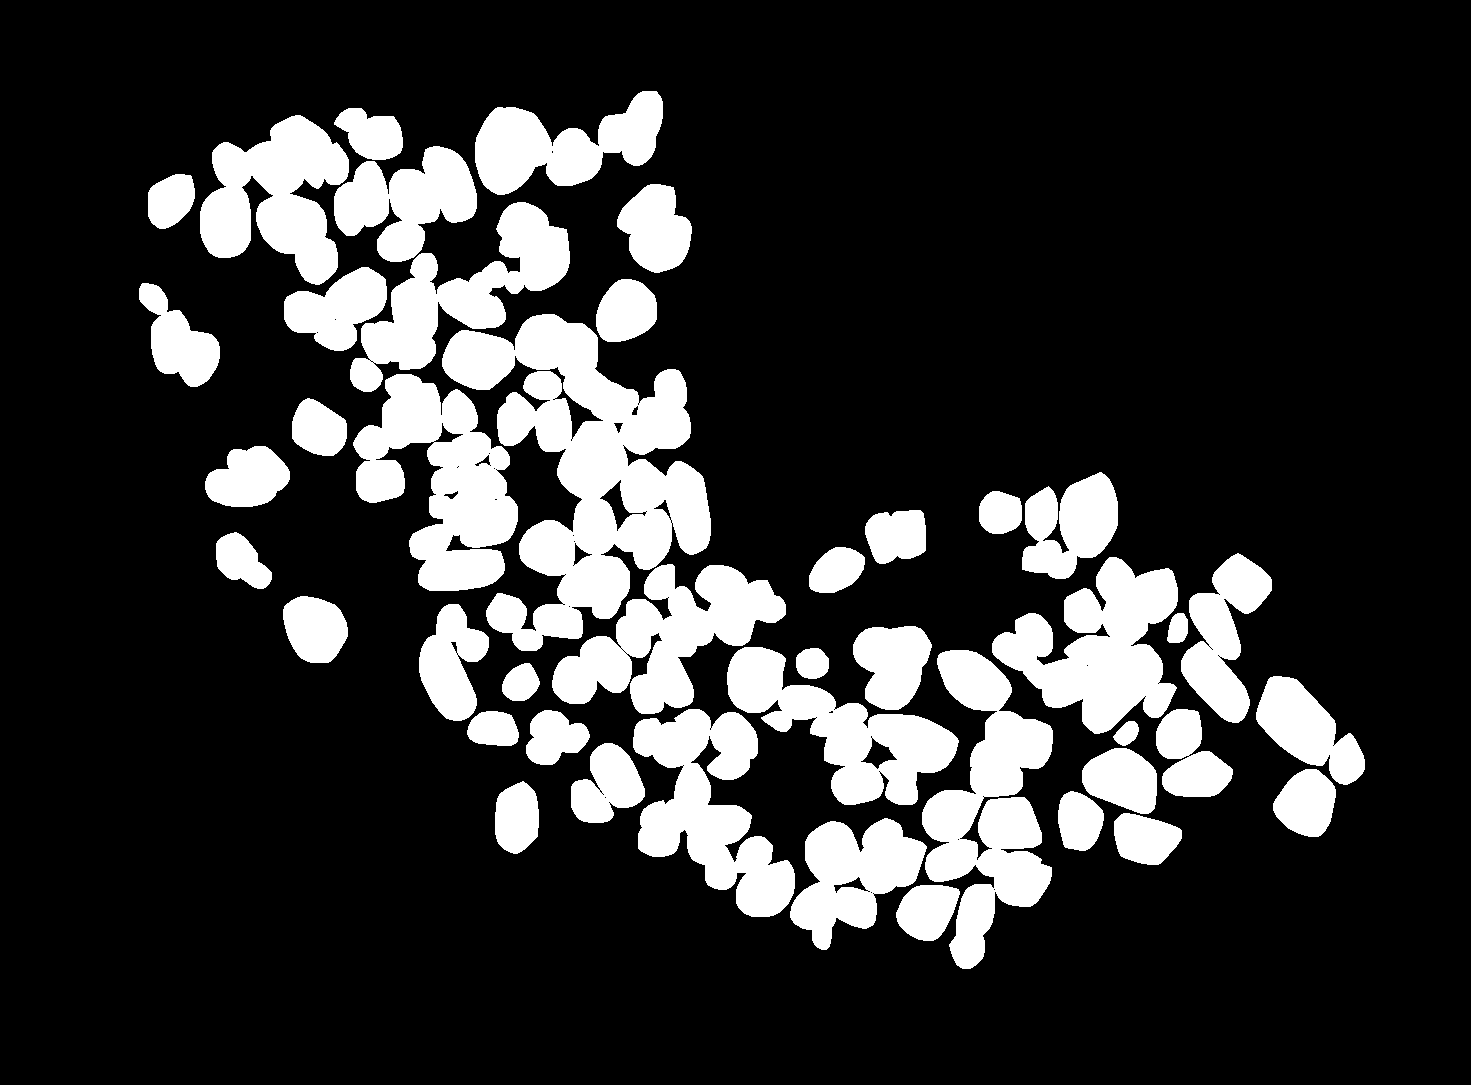
\includegraphics[width=0.5\linewidth]{realimage08.png}
    }
    
    \caption[]{
        Examples of the real data images.
        \label{fig:realdata}
    
    }
        
\end{figure}

\section{Examples of data images2}

\begin{figure}[ht]
    \centering
    \subfloat[][]{
        
\includegraphics[width=0.5\linewidth]{img001.png}
    }
    \subfloat[][]{
        
\includegraphics[width=0.5\linewidth]{img002.png}
    }
    \\
    \subfloat[][]{
        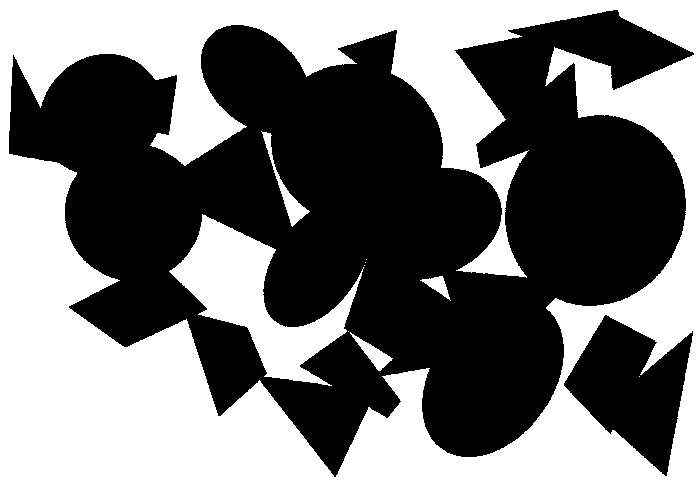
\includegraphics[width=0.5\linewidth]{img003.png}
    }
    \subfloat[][]{
        
\includegraphics[width=0.5\linewidth]{img004.png}
    }
    \\
    \subfloat[][]{
        
\includegraphics[width=0.5\linewidth]{img005.png}
    }
    \subfloat[][]{
        
\includegraphics[width=0.5\linewidth]{img006.png}
    }
    
    \caption[]{
        Examples of the synthetic data images.
        \label{fig:syntheticdata}
    
    }
        
\end{figure}

\end{document}